%\documentclass[a4paper,12pt]{book}
\documentclass[letterpaper,11pt,oneside]{book}
\usepackage[lmargin=2.5cm,
rmargin=2.5cm,top=2.7cm,bottom=3.3cm]{geometry}

\usepackage[spanish]{babel} 
\usepackage[utf8]{inputenc}
\usepackage{amsmath}
\usepackage{graphicx}
\usepackage{graphics}
\usepackage{enumitem}
\usepackage{pdfpages}

\usepackage{cancel}
\usepackage[most]{tcolorbox}
\usepackage{multicol}

\usepackage{pgf,tikz,pgfplots}
\pgfplotsset{compat=1.15}
\usepackage{mathrsfs}
\usetikzlibrary{arrows}
%\usepackage{fontspec}

\usepackage{gensymb}
\usepackage{hyperref}
%\usepackage[bookmarksnumbered=true]{hyperref}
\usepackage{bookmark,blindtext}
\usepackage{float}
\usepackage{tikz}
%\usepackage[spanish,es-noshorthands]{babel}
\usepackage{xcolor}
\usepackage{amsthm}
\usepackage{amsfonts}
%\usepackage[shortlabels]{enumitem}
%\usepackage{multicol}
%\usepackage{pdfpages}
%\usepackage[centering,text ={18 cm ,22 cm } , showframe = false]{geometry}

\usepackage{xparse} % paquete para hacer entornos con p a r m e t r o s

%Para que salgan las subsubsection en el indice
\setcounter{tocdepth}{4} 
\setcounter{secnumdepth}{4}

%para que salgan numeros en booksmarks pdf
\bookmarksetup{
	numbered,
	addtohook={%
		\ifnum\bookmarkget{level}>1 %
		\bookmarksetup{numbered=false}%
		\fi
	},
}

\newtheoremstyle{break}
{\topsep}{\topsep}%
{\itshape}{}%
{\bfseries}{}%
{\newline}{}%

\theoremstyle{definition}
\newtheorem{exer}{$\textit{\textbf{Ejercicio}}$}[section]
\newtheorem{exers}{Ejercicios}[chapter]
\newtheorem{ejemplo}{{ Ejemplo }}[section]

%\theoremstyle{theorem}
\newtheorem{theorem}{{ Teorema }}[chapter]
\newtheorem{prop}{{ Propiedad }}[chapter]
\newtheorem{defi}{{\underline{\bf Definición}}}[chapter]
\newtheorem{problem}{\textbf{\textit Problema}}[chapter]
\theoremstyle{remark}
\newtheorem{act}{ \textbf{Actividad} }[section]


\newcommand{\saleASolution}[1]{\begin{flushright} \hyperlink{#1}{\faLightbulbO} \end{flushright}}
\newcommand{\entraASolution}[1]{\hypertarget{#1}{}}

\newcommand{\saleAEjercicios}[1]{\begin{flushright} \hyperlink{#1}{\faEdit} \end{flushright}}
\newcommand{\entraAEjercicios}[1]{\hypertarget{#1}{}}

    

\begin{document}

\begin{titlepage}
\begin{center}
\begin{Huge}
\textsc{Notas de un curso de Olimpiadas}
\end{Huge}
\end{center}
\end{titlepage}

\newpage
$\ $
\thispagestyle{empty} % para que no se numere esta pagina

\chapter*{}
\pagenumbering{Roman} % para comenzar la numeracion de paginas en numeros romanos
\begin{flushright}
\textit{Grupo de Educación y Formación Matemática}
\end{flushright}

\newpage
$\ $
\thispagestyle{empty}


\tableofcontents

\newpage
$\ $
\thispagestyle{empty} % para que no se numere esta pagina

\pagenumbering{arabic} % para empezar la numeración con números
 
\part{Conteo y probabilidad}\label{cap.conteo y probabilidad}
	%\input{Combinatoria/Combinaciones_Simples/combinaciones_simples.tex}
	\chapter{Combinaciones Simples}

\begin{ejemplo}
El Club de matemáticas consta de 4 participantes y se quiere elegir un grupo de 2 personas para que vayan a competir a unas Olimpiadas. ¿De cuántas maneras se puede elegir este grupo?
\end{ejemplo}

\textit{Solución.} Digamos que estas personas se llaman Aleja, Bob, Carlos y Daniel. \textit{HACER} un diagrama de árbol para ver todas las parejas posibles. Usando el Principio de Multiplicación también podemos contar las formas de armar una fila con 2 personas, pues hay 4 opciones para elegir una persona y 3 para elegir la otra. Es decir que nos quedan 12 parejas. Que son las del diagrama de árbol (\textit{MOSTRAR}). Pero debemos fijarnos que la pareja de \textit{Aleja y Bob} (\textit{SEÑALAR}) es la misma pareja \textit{Bob y Aleja} (\textit{SEÑALAR}) y la pareja \textit{Bob y Daniel} (\textit{SEÑALAR}) es la misma pareja de \textit{Daniel y Bob}(\textit{SEÑALAR}). Así que debemos eliminar estas parejas repetidas. Es decir, del total debemos eliminar la mitad porque estoy contando 2 veces las mismas cosas (\textit{SEÑALAR} con el mismo color las iguales). Así que habrían $\frac{12}{2}=6$ grupos distintos.

\begin{ejemplo}
Si ahora fueran 5 integrantes en el Club llamados Ana (A), Beto (B), Carlos (C), Daniel (D) y Elisa (E) y se quiere llevar un grupo de 3 a la Olimpiada. ¿De cuántas maneras se pueden elegir estos 3 integrantes?
\label{integrantesclubcombinaciones}
\end{ejemplo}

\textit{Solución. }Supongamos que para ir al museo haremos una fila con los 3 integrantes antes de salir a la Olimpiada. Usando el Principio de Multiplicación habrían $5\times 4\times 3=60$ formas de hacerlo. (\textit{HACER} la lista de los 60 usando el diagrama de árbol). Pero es lo mismo la fila con A-B-C que la fila A-C-B, B-A-C, B-C-A, C-A-B, C-B-A. Es decir, que cada fila de 3 personas lo estoy contando 6 veces. (\textit{SEÑALAR} los que son iguales con el mismo color). Por tanto, la cantidad de grupos distintos de 3 integrantes del club que se pueden elegir de los 5 integrantes es $\frac{60}{6}=10$.

\begin{defi}{Combinación.\\}
En general, si se tiene un grupo con $n$ elementos y se quieren elegir $k$ de ellos. Esto se puede hacer de la siguiente cantidad de maneras $$\frac{n\cdot(n-1)\cdots (n-k+1)}{k!},$$ El siguiente número también es conocido como \textbf{n combinado k} y se denota de la siguiente manera $$ \binom{n}{k}=\frac{n\cdot(n-1)\cdots (n-k+1)}{k!}$$
\label{Combinaciondefi}
\end{defi}

Si ahora miramos nuevamente el ejemplo \ref{integrantesclubcombinaciones}. Se debían elegir 3 integrantes de un grupo de 5. Y por la definición \ref{Combinaciondefi}, la cantidad de formas que esto puede hacerse es 
\begin{equation*}
    \begin{split}
        \binom{5}{3} & = \frac{5\cdot 4\cdot 3}{3!}\\
                     & = \frac{5\cdot 4\cdot 3}{3\cdot 2\cdot 1}\\
                     & = 10.
    \end{split}
\end{equation*}

\begin{ejemplo}
Sea $X=\{ a,e,i,o,u \}$ el conjunto de las vocales. Escribir todos los subconjuntos de $X$ con 
    \begin{enumerate}[label=\Roman* )]
        \item 0 elementos.
        \item 1 elementos.
        \item 2 elementos.
        \item 3 elementos.
        \item 4 elementos.
        \item 5 elementos.
    \end{enumerate}
\end{ejemplo}
\vspace{0.3cm}

\textit{Solución. }\\

    \begin{itemize}
        \item Con 0 elementos hay 1 subconjunto, que es el que no tiene nada, el conjunto vacío.
        \item Con 1 elemento están los subconjuntos $\{ a\},\{ e\},\{ i\},\{ o\},\{ u\}$.
            Es decir, 5 subconjuntos distintos. 
        \item Con 2 elementos están $\{ a,e\},\{ a,i\},\{ a,o\},\{ a,u\},\{ e,i\},\{ e,o\},\{ e,u\},\{ i,o\},\{ i,u\},\{ o,u\}$. Es decir, 10 subconjuntos distintos. 
        \item Con 3 elementos están los siguientes 
                \vspace{2cm}

                    (***subconjuntos con 3***)

                \vspace{2cm}
        \item Con 4 elementos están los siguientes 
                \vspace{2cm}

                    (***subconjuntos con 4***)

                \vspace{2cm}
        \item Con 5 elementos sería  
                
    \end{itemize}
    
\section{Ejercicios de Combinaciones Simples}
\begin{enumerate}
    \item Un equipo de fútbol está confirmado por 11 jugadores. Un ojeador del Barcelona ha decidido llevarse a 4 jugadores a España. ¿De cuántas maneras distintas puede elegir a estos 4 jugadores?
    \item ¿Cuántos números distintos de cinco cifras se pueden formar usando tres unos y dos cuatros?
    \item **20**
    \item ***21***
    \item 
\end{enumerate}


\part{Geometría}\label{capGeometria}
	\chapter{Semejanza de Triángulos}

\rule{\textwidth}{0.1mm}
\begin{act}
	Construir en geogebra un lado $AB$ y luego construir otro lado $CD$ que sea el triple que este (Mejor si logra crear un deslizador para el valor de la razón incluso si logra crear un deslizador).
\end{act}
\rule{\textwidth}{0.1mm}

Observen laA siguiente figura

\begin{figure}[H]
	\centering
	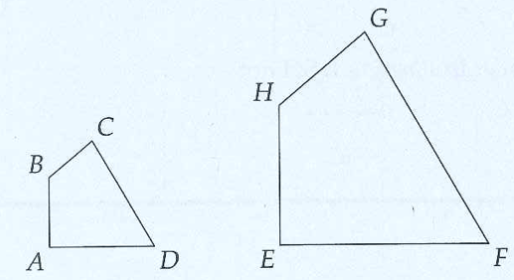
\includegraphics[width=0.7\linewidth]{Geometria/imgs/aops_geo_cuadrilateros_semejates}
	\caption{Dos cuadriláteros Semejantes}
	\label{semejanza_cuadrilateros}
\end{figure}



Podemos empezar a comparar lados, como? 

Si tu edad es 15 y la mía 30, pues $\frac{30}{15}=2$ es la cantidad de veces que mi edad supera a la tuya o \textbf{mi edad es el doble que la tuya} o \textbf{La razón entre nuestras edades es 2}. \textit{Y si yo tuviera 20 ? } : la razón entre ellas sería $\frac{20}{15}=\frac{4}{3}$.

Volviendo a nuestra figura \ref{semejanza_cuadrilateros}, \textit{Que creen que pasa con la razón entre los lados?} :  La razón entre \textbf{lados correspondientes} es la misma. Entonces en este caso 


\[
	\frac{AB}{EH} = \frac{BC}{HG} = \frac{CD}{GF} = \frac{DA}{FE}
\]

Se dice entonces que  $ABCD$ y $EFGH$ son semejantes esto es

\[ ABCD \sim EFGH
\]

\textbf{OJO.} Es importante el orden!

\rule{\textwidth}{0.1mm}
\begin{act}
	Construir en geogebra un triángulo $\triangle ABC$ y luego construir otro $\triangle YXZ$ que sea el triple que este (Mejor si logra que no importe si se mueven los vértices, se puede usar la herramienta segmento con longitud dada por ejemplo).
\end{act}
\rule{\textwidth}{0.1mm}

\begin{exer}{\ \\}
	\begin{enumerate} 
		\item (5.1.1 de \cite{Aops_Geometria}). Dados dos triángulos semejantes $\triangle ABC \sim \triangle YXZ$ cuáles de las siguientes afirmaciones son verdaderas?
		\begin{enumerate}[label=\Alph*)]
			\item $\frac{AB}{YC}=\frac{AC}{YZ}$
			\item$\frac{AB}{BC}=\frac{YX}{XZ}$
			\item $\frac{AB}{XZ}=\frac{BC}{YX}$
			\item $AC\cdot YX = YZ \cdot BA$
			\item $\frac{BC}{BA}=\frac{XY}{ZY}$
		\end{enumerate}
		\item  (5.1.2 de \cite{Aops_Geometria}). Si $\triangle ABC \sim \triangle ADB$, $AC=4cm$ y $AD=9cm$. Cuánto mide $AB$?
	\end{enumerate}
\end{exer}


\begin{theorem} \textbf{(Semejanza AA)}
	Si dos triángulos tienen dos ángulos correspondientes iguales, entonces los triángulos son semejantes. 
	\begin{figure}[H]
		\centering
		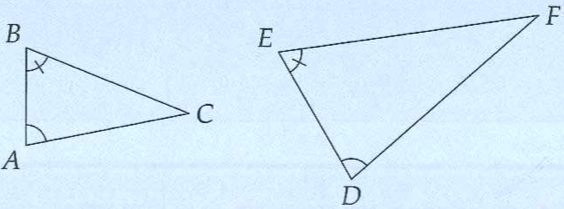
\includegraphics[width=0.7\linewidth]{Geometria/imgs/aops_geo_AA_semejanza}
		\caption{$\triangle ABC \sim \triangle DEF$ por el criterio de semejanza AA. }
		\label{teorema_aa_triangulossemejantes}
	\end{figure}
	Como $\angle A = \angle D$ y $\angle B = \angle E$ entonces $\triangle ABC \sim \triangle DEF$ y por tanto
	\[
		\frac{AB}{DE}=\frac{AC}{DF}=\frac{BC}{EF}
	\]
\end{theorem}

La demostración de este Teorema se verá mas adelane, ahora se puede ver en que problemas y cómo podemos usarlo.
\newpage




\begin{center}
	\vspace{-1cm}
	\section{ Ejercicios: Semejanza AA}
\end{center}

\begin{enumerate}
	\item \label{50_60_LAL} (5.2 de \cite{Aops_Geometria}). En la Figura \ref{semejanza5060ala}, encontrar las razones $\frac{AB}{DF}$, $\frac{AC}{DE}$, $\frac{BC}{EF}$ midiendi con una regla
	\begin{figure}[htbp]
		\centering
		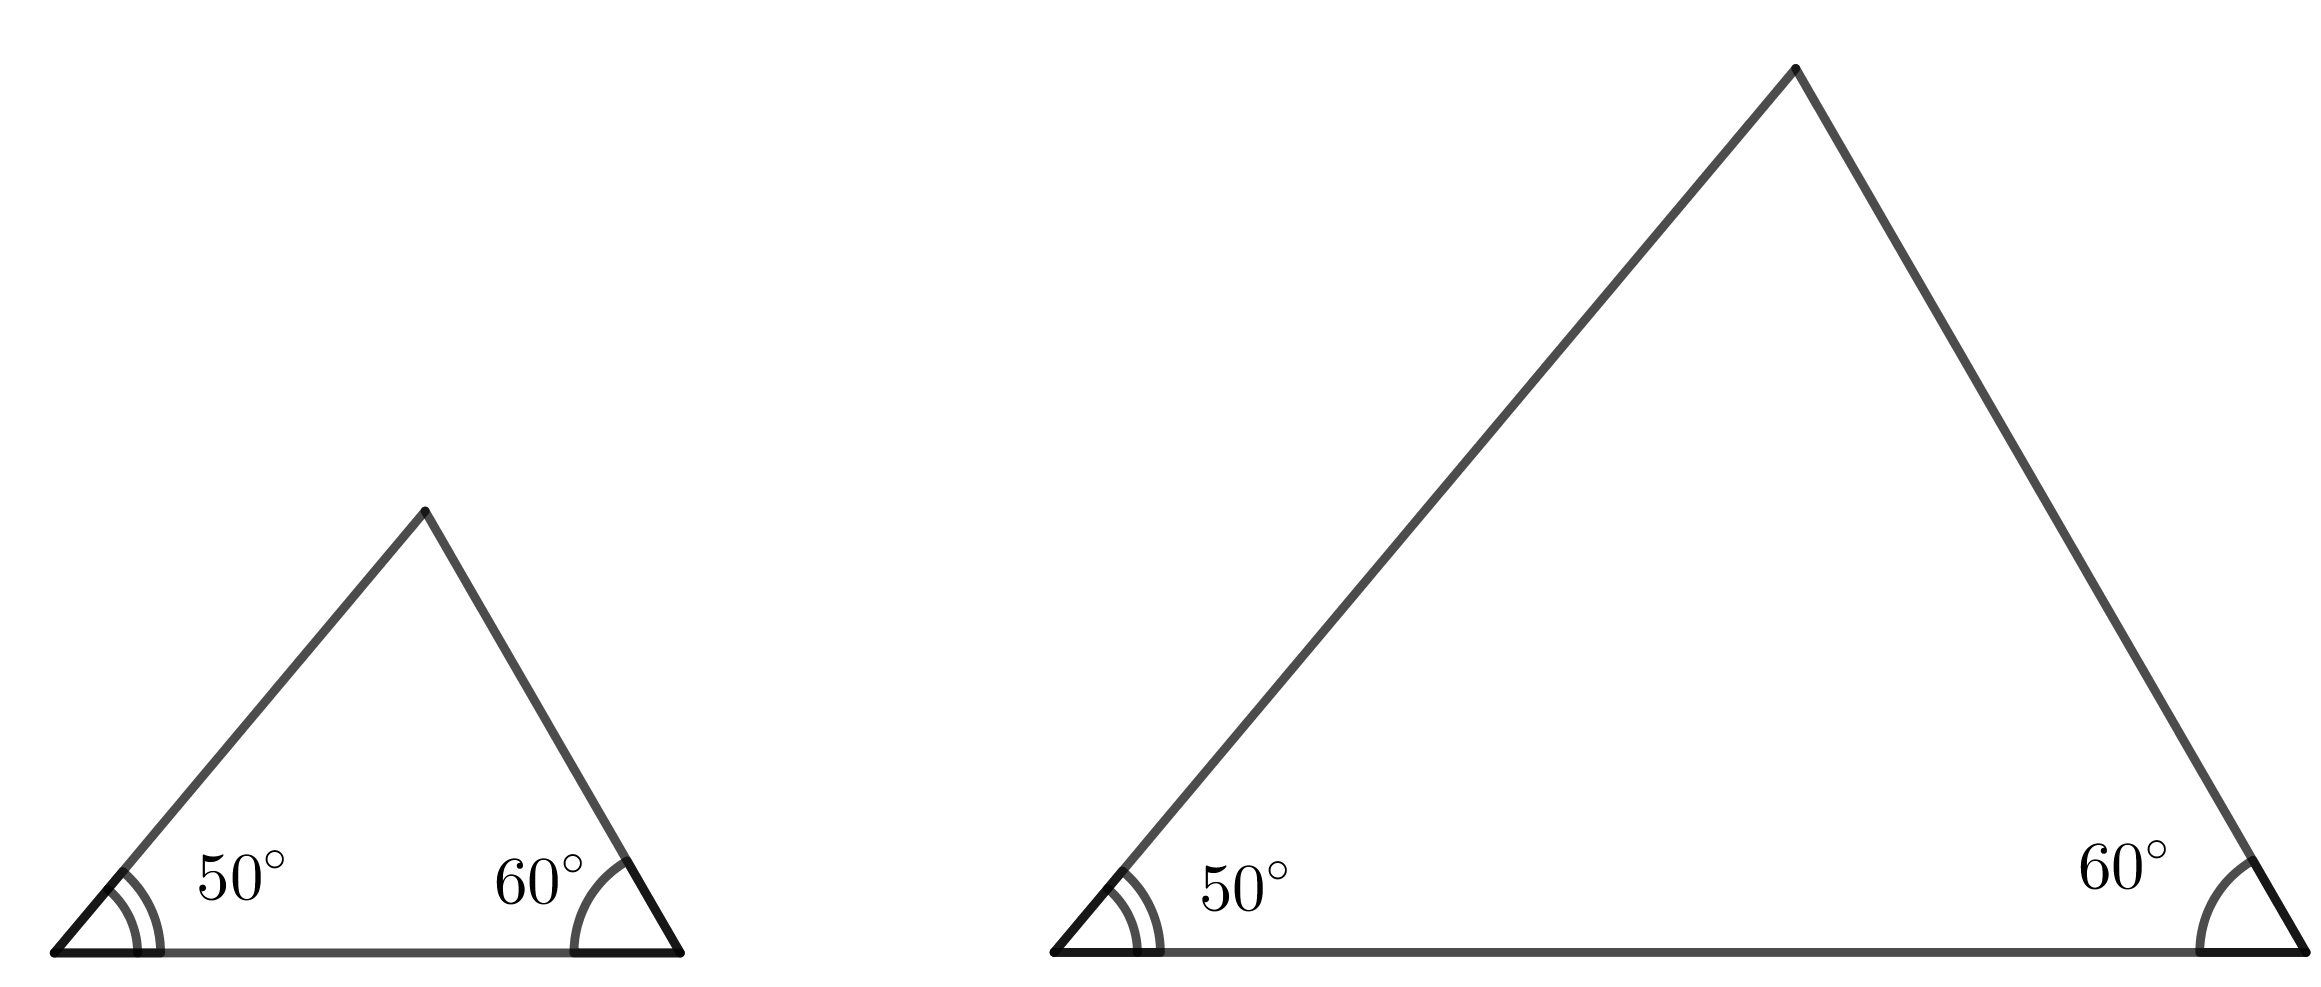
\includegraphics[width=0.7\linewidth]{Geometria/imgs/Semejanza_50_60_ALA}
		\caption{Figura del Problema \ref{50_60_LAL}. }
		\label{semejanza5060ala}
	\end{figure} 
\item (5.3 de \cite{Aops_Geometria}). El criterio AA servirá para cuadriláteros? Es decir, si $ABCD$ y $EFGH$ tienen los mismos ángulos entonces son semejantes? Si o no? Por qué?

\item \label{p5_4_aops_geo}(5.4 de \cite{Aops_Geometria}). Encontrar $MN$ (ver Figura \ref{aops_geo_p5_4} )
	\begin{figure}[H]
		\centering
		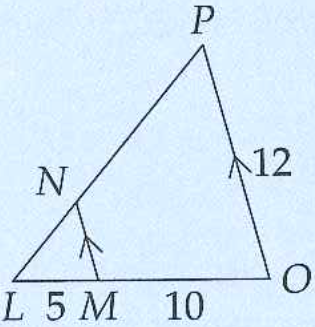
\includegraphics[width=0.25\linewidth]{Geometria/imgs/aops_geo_p5_4}
		\caption{Problema del ejercicio \ref{p5_4_aops_geo}}
		\label{aops_geo_p5_4}
	\end{figure}

\item ( p.310 de \cite{clemens}). Resolver los siguientes ejercicios


	\begin{figure}[th]
		\centering
		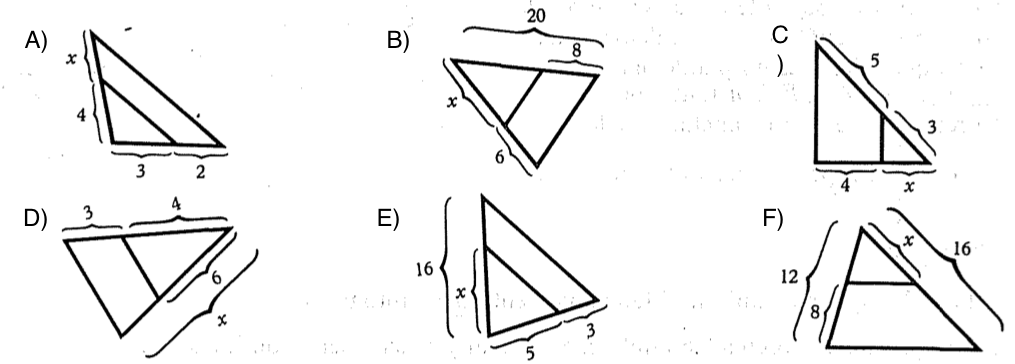
\includegraphics[width=0.87\linewidth]{Geometria/imgs/clemens_p310_3to8.png}
		\caption{}
		\label{clemens_p310_3to8}
	\end{figure}

\item \label{p5_5_aops_geo}(5.5 de \cite{Aops_Geometria}) Hallar $PY$ y $WX$ (ver Figura \ref{aops_geo_p5_5} )
	\begin{figure}[H]
		\centering
		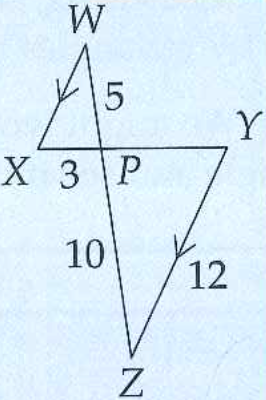
\includegraphics[width=0.25\linewidth]{Geometria/imgs/aops_geo_p5_5}
		\caption{Problema del ejercicio \ref{p5_5_aops_geo}}
		\label{aops_geo_p5_5}
	\end{figure}

\item \label{p5_6_aops_geo}(5.6 de \cite{Aops_Geometria}) Hallar $BC$ y $DC$ (ver Figura \ref{aops_geo_p5_6} )
\begin{figure}[H]
	\centering
	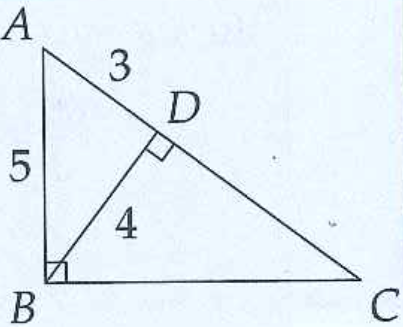
\includegraphics[width=0.25\linewidth]{Geometria/imgs/aops_geo_p5_6}
	\caption{Problema del ejercicio \ref{p5_6_aops_geo}}
	\label{aops_geo_p5_6}
\end{figure}

\item (UIS Clasificatoria Avanzado 2013) 
	\begin{figure}[H]
		\centering
		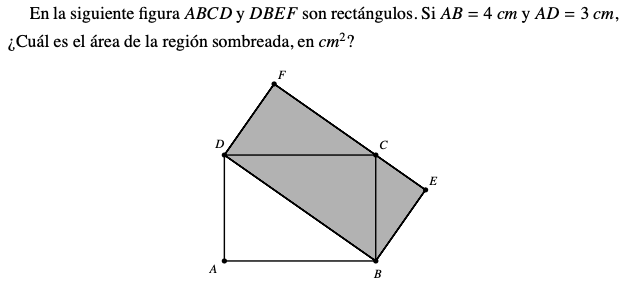
\includegraphics[width=0.9\linewidth]{Geometria/imgs/uis_2013_casi_avanzado}
		%\caption{}
		\label{uis_2013_casi_avanzado.png}
	\end{figure}
\end{enumerate}
\newpage

\begin{theorem}
	\label{teorema_paralela_en_un_triangulo}En un triángulo $\triangle ABC$, si $D$ y $E$ están entre $AB$ y $BC$ respectivamente y además $DE||AC$, entonces
	 \begin{equation*}
		\frac{AD}{DB}=\frac{EC}{BE}
	 \end{equation*}	 	
	Es decir la paralela divide a los lados proporcionalmente. 
\end{theorem}

\textbf{\textit{Esto para qué?}}
\begin{ejemplo}
	\label{ejemplo_dividir_lado_e_tres}
	Dado un segmento, solamente usando regla (sin medir) y compás dividir un segmento en 5 partes iguales.
	
	\begin{figure}[H]
		\centering
		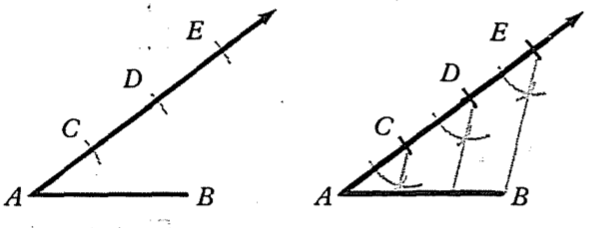
\includegraphics[width=0.7\linewidth]{Geometria/imgs/clemens_dividir_lado_en_tres}
		\caption{Ejemplo \ref{ejemplo_dividir_lado_e_tres}}
		\label{clemens_dividir_lado_en_tres}
	\end{figure}
	
\end{ejemplo}

\textit{Para probar la reciproca del Teorema \ref{teorema_paralela_en_un_triangulo} ver antes este ejemplo:}

\begin{ejemplo}\label{Ejemplo_aops_p_5_9}
	(5.9 de \cite{Aops_Geometria}) En la Figura \ref{aops_geo_p_5_9}, se tiene que 
	\[
		\frac{AB}{AC} = \frac{AD}{AE} = \frac{4}{5},
	\]
	probar que $BD||CE$.\\
	\textbf{Rta:} Note que si $BD||CE$ ya está por criterio AA. Suponiendo un segmento $BX||CE$ se puede llegar a que $AX=12$ y por tanto $X$ es $D$ y así $BD||CE$.
	
	
	\begin{figure}[H]
		\centering
		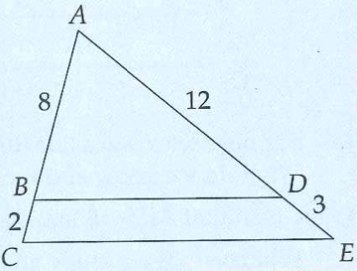
\includegraphics[width=0.5\linewidth]{Geometria/imgs/aops_geo_p_5_9}
		\caption{Figura del ejemplo \ref{Ejemplo_aops_p_5_9}.}
		\label{aops_geo_p_5_9}
	\end{figure}
\end{ejemplo}







Con el anterior ejemplo se pueden intentar probar el siguiente teorema.

\begin{theorem}
	(Reciproca del Teorema \ref{teorema_paralela_en_un_triangulo} ). En un triángulo $\triangle ABC$, si $D$ y $E$ están entre $AB$ y $BC$ respectivamente tal que
	\begin{equation*}
	\frac{AD}{DB}=\frac{EC}{BE}
	\end{equation*}	 	
	entonces $DE||AC$. 
\end{theorem}


\begin{ejemplo}{(5.6 de \cite{Aops_Geometria}). \\}
	\item \label{p5_7_aops_geo} Probar que $\frac{EY}{EX} = \frac{AD}{DB}$ (ver Figura \ref{aops_geo_p5_7} )
	\begin{figure}[H]
		\centering
		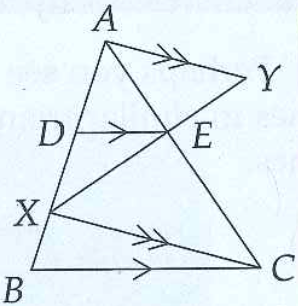
\includegraphics[width=0.25\linewidth]{Geometria/imgs/aops_geo_p5_7}
		\caption{Problema del ejermplo \ref{p5_7_aops_geo}}
		\label{aops_geo_p5_7}
	\end{figure}
	
\end{ejemplo}

\begin{exer}{\ \\}
	\item Realizar las siguientes actividades (tomadas de \cite{clemens}) menos el 15,16 y las actividades del final.
	
		\setlength{\voffset}{0cm}
		\setlength{\hoffset}{-1cm}
		
		\includepdf[pages=328,pagecommand={},width=1\textwidth]{/Users/juanolmos/MEGA/Olimpiadas/Libros/GEOMETRIA_CLEMENS_FINALLL.pdf}
		
		\setlength{\voffset}{0cm}
		\setlength{\hoffset}{-1cm}
		
		\includepdf[pages=329,pagecommand={},width=1\textwidth]{/Users/juanolmos/MEGA/Olimpiadas/Libros/GEOMETRIA_CLEMENS_FINALLL.pdf}
		
		\setlength{\voffset}{0cm}
		\setlength{\hoffset}{-1cm}
		
		\includepdf[pages=330,pagecommand={},width=1\textwidth]{/Users/juanolmos/MEGA/Olimpiadas/Libros/GEOMETRIA_CLEMENS_FINALLL.pdf}

\end{exer}


\newpage
\begin{center}
	\vspace{-1cm}
	\section{ Ejercicios: Semejanza AA}
\end{center}

\begin{exer}{\ \\}	
\begin{enumerate}
	\item (5.2.1 de \cite{Aops_Geometria}) Realizar los siguientes ejercicios 
	\begin{enumerate}[label=\Alph*)]
		 \item Hallar $AC$ y $BC$ en la Figura A) .
		
		\item  Hallar $HJ$ en la Figura B) .
		
		\item  Hallar $ON$ y $MN$ en la Figura C).
		
		\item Hallar $RS$ en la Figura D) .
		
			\begin{figure}[H]
				\centering
				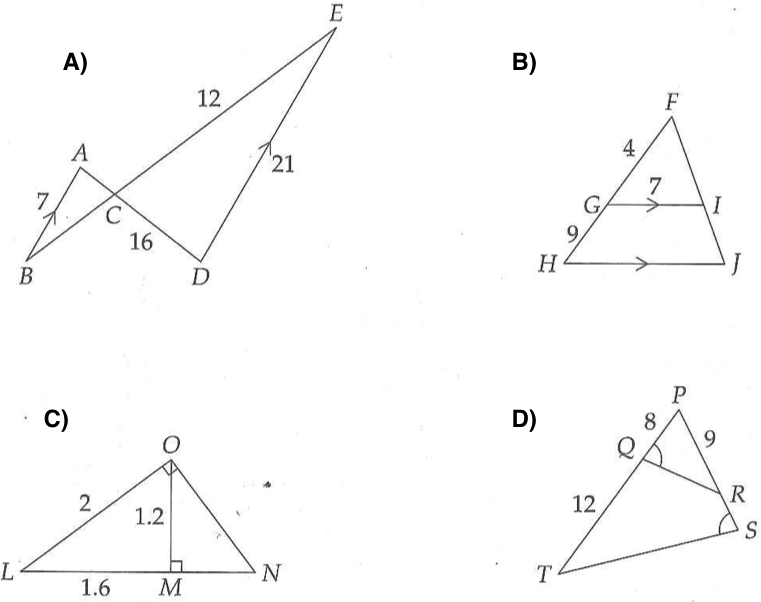
\includegraphics[width=0.7\linewidth]{Geometria/imgs/aops_geo_5_2_1}
				%\caption{Problema}
				\label{aops_geo_5_2_1}
			\end{figure}
	\end{enumerate}
	
	\item \label{p_5_2_3_aopgeo}(5.2.3 de \cite{Aops_Geometria}) En la Figura \ref{aops_geo_5_2_3} $WXYZ$ es un cuadrado. $M$ es punto medio de $YZ$ y $AB\bot MX$.
		\begin{figure}[H]
			\centering
			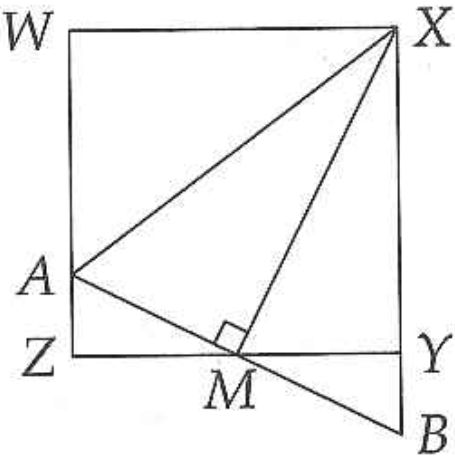
\includegraphics[width=0.3\linewidth]{Geometria/imgs/aops_geo_5_2_3}
			\caption{Problema \ref{p_5_2_3_aopgeo} }
			\label{aops_geo_5_2_3}
		\end{figure}

	
	\begin{enumerate}[label=\Alph*)]
		\item Mostrar que $WZ||XY$.
		\item Probar que $AZ=YB$.
		\item Probar que $XB=XA$.
		\item Probar que $\triangle AZM\sim \triangle MYX$ y usar esto para probar que $AZ=\frac{1}{4} XY$.
	\end{enumerate}

	\item (5.2.4 de \cite{Aops_Geometria}). En $\triangle ABC$, $AB=AC$, $BC=1$ y $\angle BAC = 36 \degree$. Sea $D$ sobre $AC$ tal que $\angle ABD = \angle CBD$.
	\begin{enumerate}[label=\Alph*)]
		\item Mostrar que $\triangle ABC\sim \triangle BCD$.
		\item\textbf{(Wow)} Hallar $AB$.
	\end{enumerate}
	
	\item \label{p_5_2_5_aopgeo} (5.2.5 de \cite{Aops_Geometria}) \textbf{Woow}. Encontrar $x$ en terminos de $y$ dado el diagrama de la Figura \ref{aops_geo_5_2_5}.
	\begin{figure}[H]
		\centering
		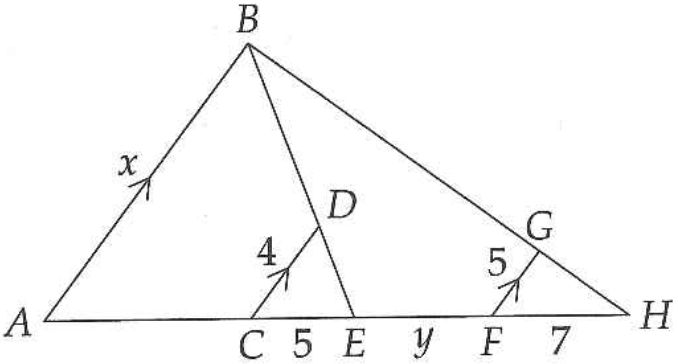
\includegraphics[width=0.5\linewidth]{Geometria/imgs/aops_geo_5_2_5}
		\caption{Problema \ref{p_5_2_5_aopgeo} }
		\label{aops_geo_5_2_5}
	\end{figure}
\end{enumerate}
	
\end{exer}

\newpage
\begin{ejemplo}
	\label{teorema_bisectriz}
	(\textbf{Teorema de la bisectriz}). En un $\triangle ABC$ al trazar la bisectriz de $\angle A $ esta intersecta al lado $BC$ en $D$ de forma que 
	\[
		\frac{AB}{AC}=\frac{BD}{DC}
	\].\\
	\textbf{Rta:} Prolongar la bisectriz hasta un punto $E$ de forma que $EC=AC$ y ver semejanzas.
\end{ejemplo}

\begin{ejemplo}
	\label{teorema_altura_en_triangulo_rectangulo}
	(\textbf{Teorema altura en un triángulo rectángulo}). Sea $\triangle ABC$ un triángulo rectángulo donde $\angle A= 90\degree $, sea $D$ la base de la altura del vértice $A$. Probar que
	\[
		BD\cdot DC = {AD}^2
	\]
	\textbf{Rta:} Ver la semejanza $\triangle ABC \sim \triangle DBA$. Otra solución es por pitágoras, ver ambas.
\end{ejemplo}

\section{Criterio LAL}
\begin{theorem} \textbf{(Semejanza LAL)}
	Si dos triángulos tienen dos lados corresponndientes proporcionales y además el ángulo entre ellos es el mismo entonces son semejantes. Es decir, si $\frac{AB}{DE} = \frac{AC}{DF}$ y $\angle A =\angle D$ entonces $\triangle ABC \sim \triangle DEF$ (Ver Figura \ref{aops_geo_criterio_LAL}).
	
	\begin{figure}[H]
		\centering
		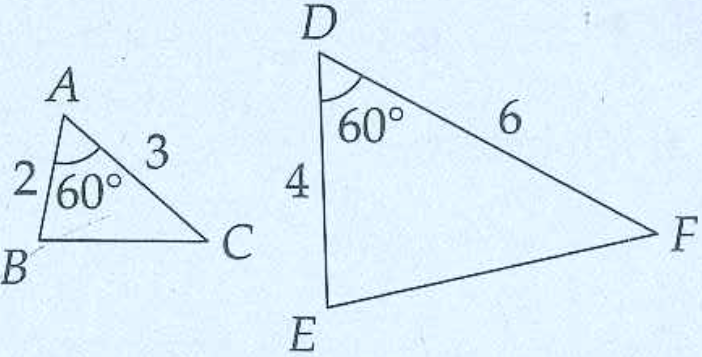
\includegraphics[width=0.5\linewidth]{Geometria/imgs/aops_geo_criterio_LAL}
		\caption{Criterio LAL}
		\label{aops_geo_criterio_LAL}
	\end{figure}
\end{theorem}

Mirar nuevamente el ejercicio \ref{aops_geo_p_5_9} y ver que $\triangle ABD \sim \triangle ACE$. \textit{Cómo se puede usar esto para probar el criterio LAL? } :Vea que sería como meter un triángulo dentro del otro.

\begin{ejemplo}
	(5.10 de \cite{Aops_Geometria} ). Hallar $BC$ si el perimetro de $\triangle BCD$ es 20 (Ver Figura \ref{aops_geo_p_5_10}).
\begin{figure}[H]\label{ej_p_5_10_aops}
	\centering
	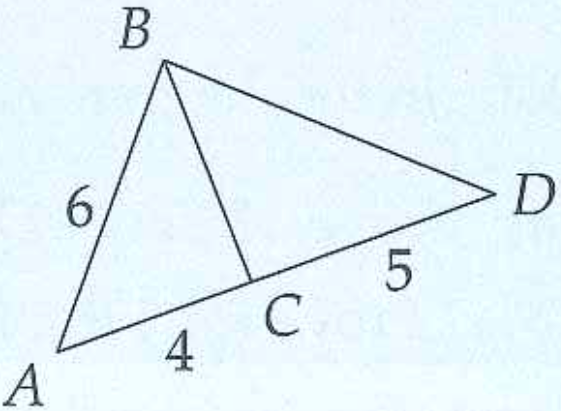
\includegraphics[width=0.3\linewidth]{Geometria/imgs/aops_geo_p_5_10}
	\caption{Ejemplo \ref{ej_p_5_10_aops}}
	\label{aops_geo_p_5_10}
\end{figure}
	\textbf{Rta:} Note que $\triangle ABC \sim \triangle ADB$ pues comparten $\angle A$ y $$\frac{AB}{AD}=\frac{AC}{AB}=\frac{2}{3},$$ entonces son semejantes por \textbf{LAL} y por tanto $\frac{BC}{BD}=\frac{2}{3}$, o sea $BC=\frac{2\cdot BD}{3}$ y así como el perimetro de $\triangle BCD=20$, entonces
	\begin{equation*}
		\begin{split}
			5+BD+BC&=20\\
			BD+\frac{2\cdot BD}{3} &= 15\\
			3BD+2BD&=45\\
			5BD&=45\\
			BD&=9,
		\end{split}
	\end{equation*}
			y así $BC=6$.
\end{ejemplo}

\rule{\textwidth}{0.1mm}
\begin{act}
	Construir en geogebra un triángulo $\triangle ABC$ y luego construir otro $\triangle YXZ$ usando el criterio LAL (Si se puede, usar deslizadores para variar la razón).
\end{act}
\rule{\textwidth}{0.1mm}

\newpage
\begin{center}
	\vspace{-1cm}
	\subsection{ Ejercicios: Semejanza LAL}
\end{center}

\begin{enumerate}
	\item \label{P531_aopgeo} (5.3.1 de \cite{Aops_Geometria}). Encontrar $DE$ en la Figura \ref{531_aopgeo}
	
		\begin{figure}[H]
			\centering
			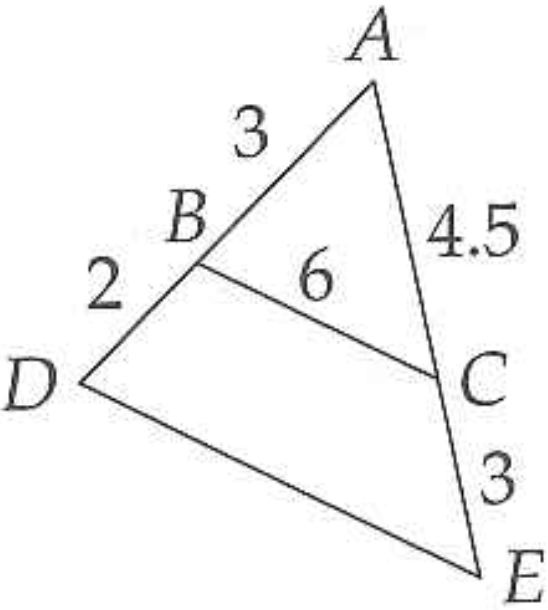
\includegraphics[width=0.2\linewidth]{Geometria/imgs/531_aopgeo}
			\caption{Ejercicio \ref{P531_aopgeo} }
			\label{531_aopgeo}
		\end{figure}
	
	\item \label{P532_aopgeo} (5.3.2 de \cite{Aops_Geometria}). En la Figura \ref{532_aopgeo}, $M$ es el punto medio de $\overline{EH}$ y $\overline{FG}$. $E$ y $F$ son puntos medios de $\overline{IM}$ y $\overline{MJ}$ respectivamente. Probar que $IJ||GH$.
	
	\begin{figure}[H]
		\centering
		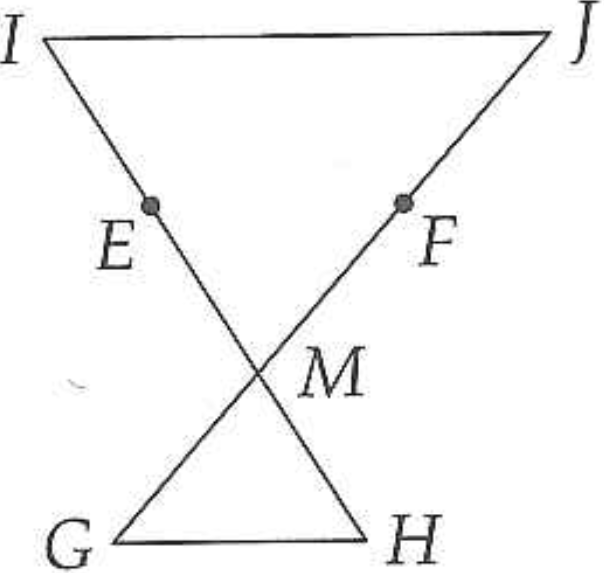
\includegraphics[width=0.25\linewidth]{Geometria/imgs/532_aopsgeo}
		\caption{Ejercicio \ref{P532_aopgeo} }
		\label{532_aopgeo}
	\end{figure}

	\item \label{P533_aopgeo} (5.3.3 de \cite{Aops_Geometria}). Mostrar que si ${WZ}^2 = (WX)(WY)$ en la Figura \ref{533_aopgeo}, entonces $\angle WZX = \angle WYZ$.
	
	\begin{figure}[H]
		\centering
		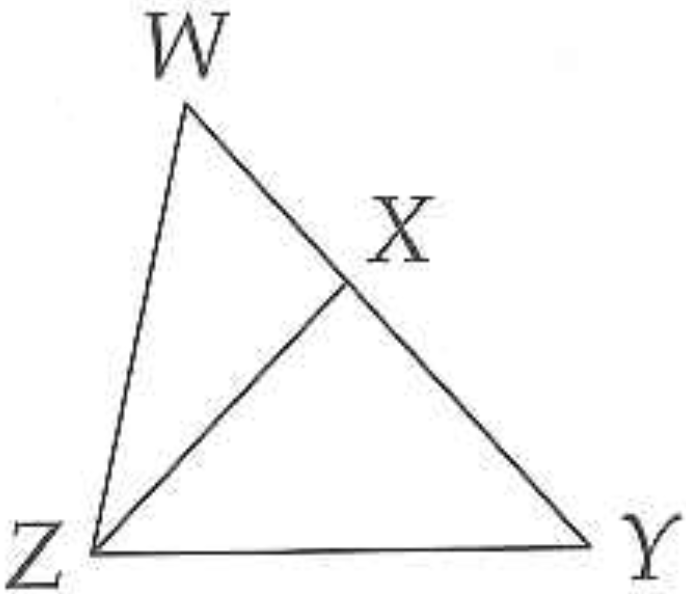
\includegraphics[width=0.25\linewidth]{Geometria/imgs/533_aopsgeo}
		\caption{Ejercicio \ref{P533_aopgeo} }
		\label{533_aopgeo}
	\end{figure}
	
	\item \label{P534_aopgeo} (5.3.4 de \cite{Aops_Geometria}). En la Figura \ref{534_aopgeo}, $\angle PRQ = \angle PQA = \angle 90\degree $, $QR=QA$ y $\angle QPC = \angle RPC$.
	\begin{enumerate}[label=\Alph*)]
			\item Probar $\angle QCB = \angle QBC$.
			\item \textbf{Wow}. Probar que $RA||PB$.
	\end{enumerate}
	
		\begin{figure}[H]
			\centering
			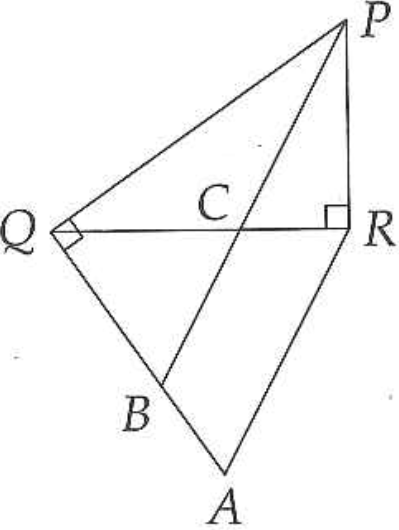
\includegraphics[width=0.25\linewidth]{Geometria/imgs/534_aopsgeo}
			\caption{Ejercicio \ref{P534_aopgeo} }
			\label{534_aopgeo}
		\end{figure}
	
	
\end{enumerate}
\newpage

\section{Criterio LLL}
\begin{theorem} \textbf{(Semejanza LLL)}
	Si dos triángulos tienen los lados corresponndientes proporcionales entonces son semejantes. Es decir, si $\frac{AB}{DE} = \frac{AC}{DF}= \frac{BC}{EF}$ entonces $\triangle ABC \sim \triangle DEF$ (Ver Figura \ref{aops_geo_criterio_LLL}).
	
	\begin{figure}[H]
		\centering
		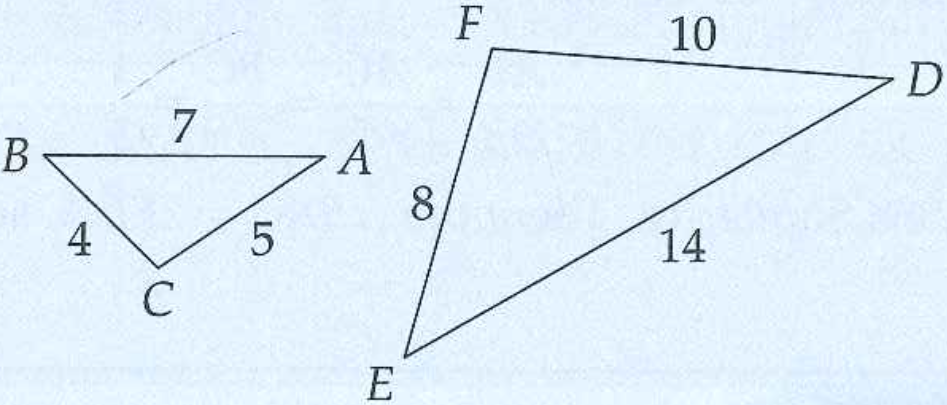
\includegraphics[width=0.5\linewidth]{Geometria/imgs/aops_geo_criterio_LLL}
		\caption{Criterio LLL}
		\label{aops_geo_criterio_LLL}
	\end{figure}
\end{theorem}

\begin{ejemplo}{(5.11 de \cite{Aops_Geometria})}
\label{ejemplo_5_11_aopsgeo}En la Figura \ref{5_11_aopsgeo} probar que $AE||BC$ y $AB||DE$.
	\begin{figure}[H]
		\centering
		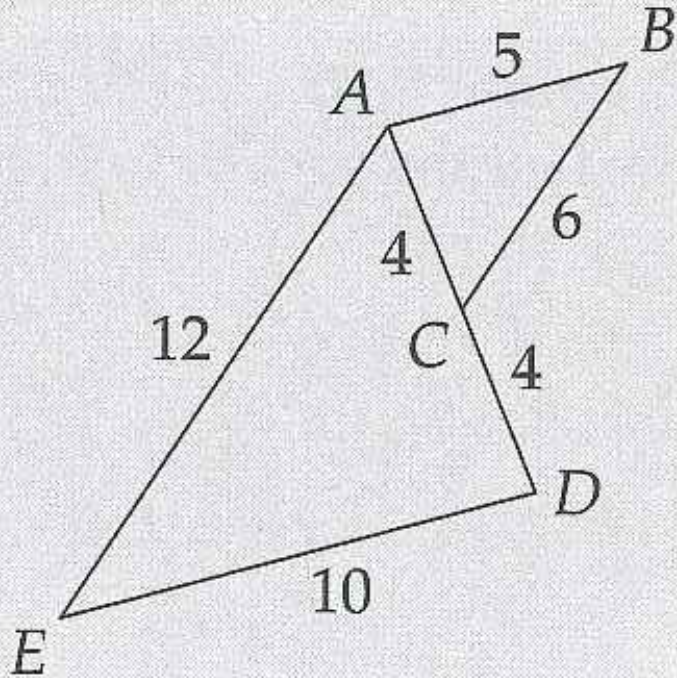
\includegraphics[width=0.3\linewidth]{Geometria/imgs/5_11_aopsgeo}
		\caption{Ejemplo \ref{ejemplo_5_11_aopsgeo}.}
		\label{5_11_aopsgeo}
	\end{figure}
		\textbf{Rta:} Para que $AE||BC$ se tiene que probar que $\angle EAD =\angle BCA$ y para probar que $AB||DE$ se tiene que probar que $\angle CAB =\angle AED$, y esto se tendría si $\triangle EAD \sim \triangle BCA$. Note que $\frac{EA}{BC}=\frac{12}{6}=2$, $\frac{ED}{BA}=\frac{10}{5}=2$ y $\frac{AD}{CA}=\frac{8}{4}=2$, es decir, son semejantes por \textbf{LLL}.
\end{ejemplo}


\begin{ejemplo}{(5.12 de \cite{Aops_Geometria})}
	\label{ejemplo_5_12_aopsgeo}En la Figura \ref{5_12_aopsgeo} se tiene que $DE||BC$. Encontrar $x,y,z$.
	\begin{figure}[H]
		\centering
		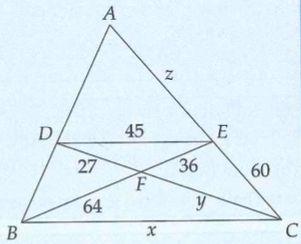
\includegraphics[width=0.3\linewidth]{Geometria/imgs/5_12_aopsgeo}
		\caption{Ejemplo \ref{ejemplo_5_12_aopsgeo}.}
		\label{5_12_aopsgeo}
	\end{figure}
		\textbf{Rta:} Con la semejanza $\triangle FED \sim \triangle FBC$ se pueden hallar $x$ e $y$. Y con la semejanza $\triangle AED \sim \triangle ACB$ se puede calcular $z$.
\end{ejemplo}

\begin{ejemplo}{(5.13 de \cite{Aops_Geometria})}
	\label{ejemplo_5_13_aopsgeo}En la Figura \ref{5_13_aopsgeo} se tiene que $AB=6$ y $AC=10$. Encontrar $AD$.
	\begin{figure}[H]
		\centering
		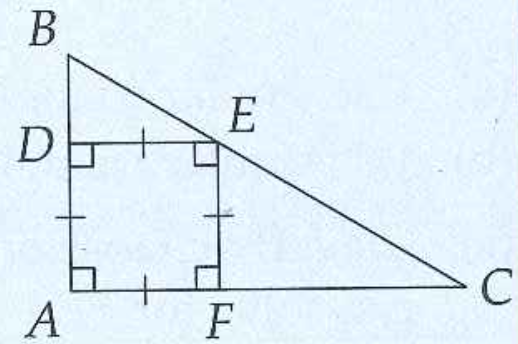
\includegraphics[width=0.3\linewidth]{Geometria/imgs/5_13_aopsgeo}
		\caption{Ejemplo \ref{ejemplo_5_13_aopsgeo}.}
		\label{5_13_aopsgeo}
	\end{figure}
	\textbf{Rta:} Dando un valor $x$ al lado del cuadrado y viendo que $\triangle BAC \sim \triangle BDE \sim \triangle EFC$.
\end{ejemplo}

\begin{ejemplo}{(5.14 de \cite{Aops_Geometria})}
	\label{ejemplo_5_14_aopsgeo}En la Figura \ref{5_14_aopsgeo} mostrar 
	\begin{enumerate}[label=\Alph*) ]
			\item ${PX}^2 = QX\cdot RX$.
			\item ${PR}^2 = RX\cdot RQ$.
			\item ${PQ}^2 = QX\cdot QR$.
	\end{enumerate}
	\begin{figure}[H]
		\centering
		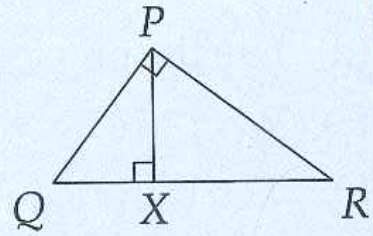
\includegraphics[width=0.3\linewidth]{Geometria/imgs/5_14_aopsgeo}
		\caption{Ejemplo \ref{ejemplo_5_14_aopsgeo}.}
		\label{5_14_aopsgeo}
	\end{figure}
\end{ejemplo}

\begin{ejemplo}{(5.15 de \cite{Aops_Geometria})}
	\label{ejemplo_5_15_aopsgeo} $\triangle ABC \sim \triangle XYZ$, $\frac{AB}{XY}=4$, y $\left[ABC\right]=64$. Hallar $\left[XYZ\right]$
	\textbf{Rta:} Sabemos que si dos triángulos son semejantes entonces las alturas tienen la misma proporción que esta semejanza. 
\end{ejemplo}

\begin{ejemplo}{(5.16 de \cite{Aops_Geometria})}
	\label{ejemplo_5_16_aopsgeo}En la Figura \ref{5_16_aopsgeo}, $P$ es el punto medio de $\overline{AB}$. Probar que $\overline{PQ}\parallel \overline{BC}$.
	\begin{figure}[H]
		\centering
		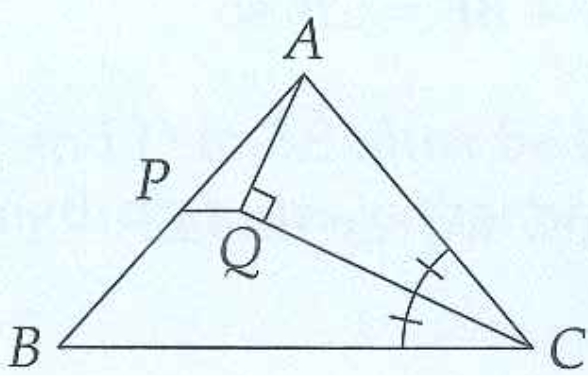
\includegraphics[width=0.3\linewidth]{Geometria/imgs/5_16_aopsgeo}
		\caption{Ejemplo \ref{ejemplo_5_16_aopsgeo}.}
		\label{5_16_aopsgeo}
	\end{figure}
	\textbf{Rta: }Si se extiende $AQ$ hasta intersectar a $BC$ en $H$, se puede ver $\triangle CQA \cong \triangle CQH$ entonces $AQ=QH$. Entonces como $\frac{AP}{AB}=\frac{AQ}{AH}=\frac{1}{2}$ entonces $\overline{PQ}\parallel \overline{BC}$ por el Teorema \ref{teorema_paralela_en_un_triangulo}.
\end{ejemplo}

\begin{ejemplo}{(5.17 de \cite{Aops_Geometria})}
	\label{ejemplo_5_17_aopsgeo}En la Figura \ref{5_17_aopsgeo}, El asta de bandera $\overline{CD}$ mide 12 metros de alto. El asta de bandera $\overline{AB}$ mide 9 metros de alto. Ambas astas son perpendiculares al piso. Un cable recto está amarrado desde $B$ hasta $D$ y otro desde $A$ hasta $C$. Las astas están separadas 40 metros y los cables se encuentran en $E$ que está justamente encima del punto $F$ que está en el piso. Hallar $EF$.
	\begin{figure}[H]
		\centering
		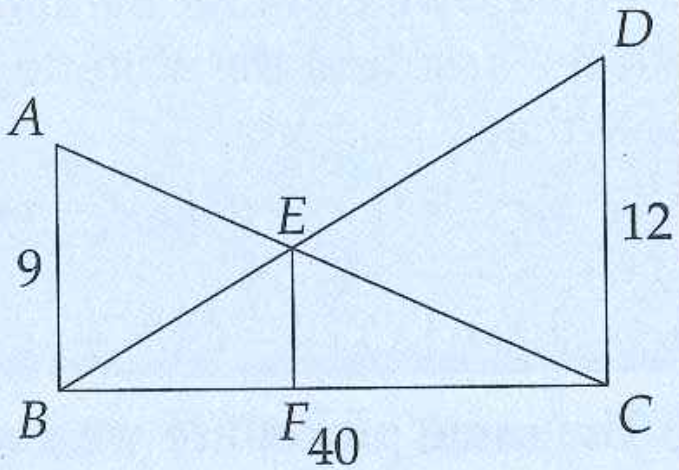
\includegraphics[width=0.3\linewidth]{Geometria/imgs/5_17_aopsgeo}
		\caption{Ejemplo \ref{ejemplo_5_17_aopsgeo}.}
		\label{5_17_aopsgeo}
	\end{figure}
	\textbf{Rta: }Note que $\triangle ABC \sim \triangle EFC$ y $\triangle DCB \sim \triangle EFB$. Opción 1, De forma algebraica tomando $EF=h$ y $FC=x$ y planteando las dos ecuaciones de la semejanza. Opción 2 no se usa que $BC=40$ \textbf{te atreves?}, de la semejanza se tiene que $$\frac{EF}{AB} = \frac{\textbf{FC}}{\textbf{BC}} = \frac{EC}{AC}\hspace{5mm}\text{ y }\hspace{5mm}\frac{EF}{DC} = \frac{\textbf{FB}}{\textbf{BC}} = \frac{EB}{DB}.$$
	Sumando las fracciones subrayadas 
	\begin{equation*}
		\begin{split}
			\frac{EF}{AB}  + \frac{EF}{DC} &= \frac{\textbf{FC}}{\textbf{BC}} + \frac{\textbf{FB}}{\textbf{BC}} \\
			\frac{EF}{AB}  + \frac{EF}{DC} &= 1 \\
			EF \left( \frac{1}{AB}  + \frac{1}{DC} \right) &=1\\
			EF \left( \frac{1}{9}  + \frac{1}{12} \right) &=1\\
			EF \frac{21}{108} &=1\\
			EF &= \frac{108}{21}\\
			EF  &= \frac{36}{7}
		\end{split}
	\end{equation*}
\end{ejemplo}

\begin{ejemplo}{(5.18 de \cite{Aops_Geometria})}
	\label{ejemplo_5_18_aopsgeo}En la Figura \ref{5_18_aopsgeo}, Hallar $BE$ y$DE$ \textbf{sin} usar el cirterio de semejanza semejanza AA.
	\begin{figure}[H]
		\centering
		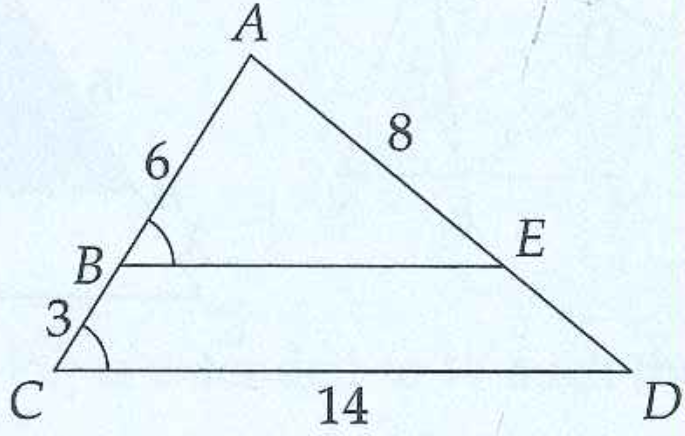
\includegraphics[width=0.5\linewidth]{Geometria/imgs/5_18_aopsgeo}
		\caption{Ejemplo \ref{ejemplo_5_18_aopsgeo}.}
		\label{5_18_aopsgeo}
	\end{figure}
	\textbf{Rta: }Queremos encontrar que relación relación $\frac{AB}{AC} = \frac{AE}{ED}$ es cierta. Una técnica útil es usar \textbf{áreas!} podemos trazar $BD$ y $CE$ (Ver figura \ref{5_18_aopsgeo_sol}) para construir triángulos que nos puedan dar esta información, pues note que la relación $\frac{AB}{AC}$ surge al comparar $[ABE]$ y $[ACE]$ ya que al tener la misma altura los triángulos $\triangle ABE$ y $\triangle ACD$, como $[ABE]=\frac{1}{2}AB\cdot h$, entonces $h=\frac{2[ABE]}{AB}$ y del $\triangle AEC$ se tiene que $h=\frac{2[ACE]}{AC}$, entonces 
	\[
		\frac{[ABE]}{[ACE]} = \frac{AB}{AC} =\frac{6}{9} = \frac{2}{3}
	\]
	Lo mismo se tiene con $\triangle ABE$ y $\triangle ABD$, tienen la misma altura y entonces 
	\[
	\frac{[ABE]}{[ABD]} = \frac{AE}{AD} =\frac{8}{8+ED} 
	\]
	\begin{figure}[H]
		\centering
		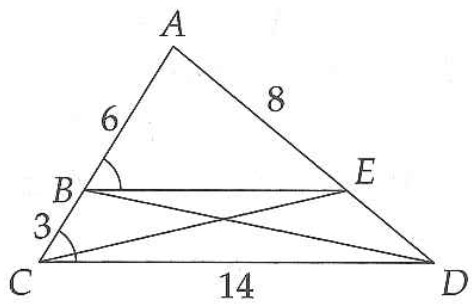
\includegraphics[width=0.5\linewidth]{Geometria/imgs/5_18_aopsgeo_sol}
		\caption{Solución de \ref{ejemplo_5_18_aopsgeo}}
		\label{5_18_aopsgeo_sol}
	\end{figure}
	Vemos entonces que si $\frac{AB}{AC} = \frac{AE}{ED}$ entonces ya podemos conocer $ED$. Necesitariamos entonces que $\frac{[ABE]}{[ACE]}=\frac{[ABE]}{[ABD]}$, es decir que $[ACE]=[ABD]$. Y esta igualdad es cierta porque se puede ver que $[BED]=[BEC]$ y como comparten $[ABD]$ entonces efectivamente $[ACE]=[ABD]$. Entonces $\frac{AB}{AC} = \frac{AE}{ED}$ y así $\frac{2}{3}=\frac{8}{8+ED} $, de donde $ED=4$.

		Para hallar $BE$ quisieramos aplicar algo parecido, entonces basta con mover el $\triangle ABE$ al vértice $D$, ver Figura \ref{5_18_aopsgeo_sol2}. Se puede ver $\triangle ABE \cong \triangle A'B'D$  para ver que $A'D=AE=8$ y que $\angle A' = \angle A$ y así tenemos el mismo problema cuando calculamos $DE$ pero girado y el problema es hallar $B'D$ pues sabemos por la congruencia que $B'D=BE$. De ese problema supimos que con solo áreas se puede probar que
		\[
			\frac{A'D}{AD} = \frac{B'D}{CD},
		\]
		es decir
		\[
			\frac{8}{12} = \frac{B'D}{14},			
		\]
		de donde se obtiene que $BE=B'D=\frac{28}{3}$.
\begin{figure}[H]
	\centering
	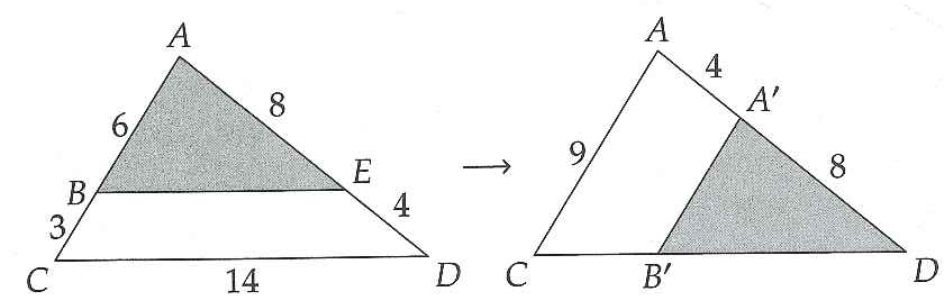
\includegraphics[width=0.7\linewidth]{Geometria/imgs/5_18_aopsgeo_sol2}
	\caption{Solución \ref{ejemplo_5_18_aopsgeo}}
	\label{5_18_aopsgeo_sol2}
\end{figure}

\end{ejemplo}

\textbf{OJO. }Es muy útil \textbf{usar áreas para hallar proporciones}, no solo sirve para calcular áreas de ciertas zonas.

\newpage
\begin{center}
	\vspace{-1cm}
	\subsection{ Ejercicios: Semejanza LLL}
\end{center}
	
\begin{enumerate}
	\item \label{P551_aopgeo_ejercicio} (5.5.1 de \cite{Aops_Geometria}). $X$ e $Y$ están en los lados $\overline{PQ}$ y $\overline{PR}$ de $\triangle PQR$ respectivamente, de forma que $XY \parallel QR$. Si $XY = 5$, $QR=15$ y $YR=8$, encontrar $PY$.
	\item \label{P552_aopgeo_ejercicio} (5.5.2 de \cite{Aops_Geometria}). $[EDC]=25[BFD]$.
			\begin{enumerate}[label=\Alph*)]
				\item Encontrar $\frac{CD}{DB}$.
				\item Encontrar $\frac{[EDC]}{[ABC]}$.
				\item \textbf{Woow} Encontrar $\frac{[AFE]}{[ABC]}$.
			\end{enumerate}
	\begin{figure}[H]
		\centering
		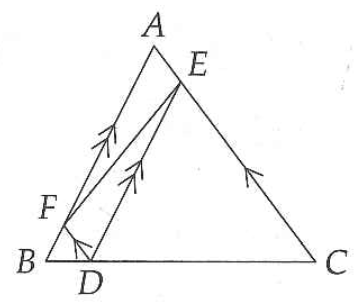
\includegraphics[width=0.4\linewidth]{Geometria/imgs/552_aopgeo_ejer}
		\caption{Ejercicio \ref{P552_aopgeo_ejercicio} }
		\label{552_aopgeo}
	\end{figure}

	\item \label{P553_aopgeo_ejercicio} (5.5.3 de \cite{Aops_Geometria}). En la Figura \ref{553_aopgeo}, $WZ\parallel XY$ y $WX\parallel ZY$, $WA$ y $WB$ intersectan a $XZ$ en $C$ y $D$ respectivamente, de forma que $ZC=XD$.
	\begin{enumerate}[label=\Alph*)]
		\item Probar que $\frac{ZC}{XC} = \frac{AC}{WC}$.
		\item Probar que $\frac{XD}{ZD} = \frac{DB}{WD}$.
		\item Probar que $CD\parallel AB$.
	\end{enumerate}
	\begin{figure}[H]
		\centering
		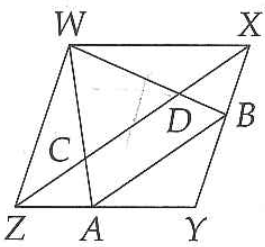
\includegraphics[width=0.3\linewidth]{Geometria/imgs/553_aopgeo_ejer}
		\caption{Ejercicio \ref{P553_aopgeo_ejercicio} }
		\label{553_aopgeo}
	\end{figure}		
	
	\item \label{P554_aopgeo_ejercicio} (5.5.4 de \cite{Aops_Geometria}). En la Figura \ref{554_aopgeo}, $PQ=PR$ y $ZX\parallel QY$
	\begin{enumerate}[label=\Alph*)]
		\item Probar que $\triangle QWZ \sim \triangle RXZ$.
		\item \textbf{Wow} Probar que $YQ = ZX-ZW$.
	\end{enumerate}
	\begin{figure}[H]
		\centering
		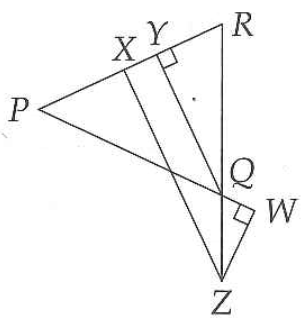
\includegraphics[width=0.3\linewidth]{Geometria/imgs/554_aopgeo_ejer}
		\caption{Ejercicio \ref{P554_aopgeo_ejercicio} }
		\label{554_aopgeo}
	\end{figure}		

	\item \label{P555_aopgeo_ejercicio} (5.5.5 de \cite{Aops_Geometria}). En la Figura \ref{555_aopgeo}, $PA$ y $QB$ son bisectrices de $\angle P$ y $\angle Q$ respectivamente. Si $RX\perp PA$ y $RY\perp BQ$, probar que $XY\parallel PQ$
	\begin{figure}[H]
		\centering
		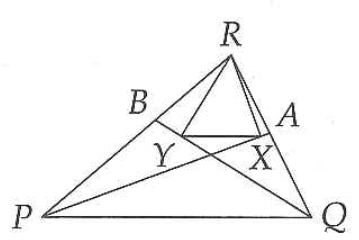
\includegraphics[width=0.3\linewidth]{Geometria/imgs/555_aopgeo_ejer}
		\caption{Ejercicio \ref{P555_aopgeo_ejercicio} }
		\label{555_aopgeo}
	\end{figure}		
	
\end{enumerate}
\newpage

\begin{center}
	\vspace{-1cm}
	\section{ Ejercicios revisión: Semejanza de triángulos}
\end{center}

	\begin{enumerate}
		\item Si dos triángulos son semejantes, probar que las alturas tienen la misma proporción, es decir si la proporción de la semejanza es $k$, entonces la proporción entre las alturas es $k$.
		
		\item Si dos triángulos son semejantes, probar que las medianas tienen la misma proporción, es decir si la proporción de la semejanza es $k$, entonces la proporción entre las medianas es $k$.
		
		\item Si dos triángulos son semejantes, probar que las bisectrices tienen la misma proporción, es decir si la proporción de la semejanza es $k$, entonces la proporción entre las bisectrices es $k$.
		
		\item Si la proporción de la semejanza entre dos triángulos es $k$, entonces la proporción entre las áreas es $k^2$.
		
		\item (Problema 2 Geometría N.2 A.4 de \cite{POTI}). En un $\triangle ABC$, $AB=4cm,BC=5cm$ y $AC=6cm$. Calcular la medida de los lados un triángulo semejante a $ABC$ que tenga perímetro $20cm$.
		
		\item (Problema 3  Geometría N.2 A.4 de \cite{POTI}). Sea $ABC$ un triángulo equilatero de lado $20cm$. Una recta pasa por el punto medio $M$ en el lado $AB$ y un punto $N$ en el lado $AC$ y corta a la recta $\overleftrightarrow{BC}$ en el punto $P$ de modo que $CP=12cm$. Hallar la longitud de $NA$.
		
		%\item (Problema 4  Geometría N.2 A.4 de \cite{POTI}). Sean $D$ y $E$ puntos sobre los lados $AB$ y $AC$ de un triangulo $ABC$ respectivamente. Si
		
		\item \label{review_P522_aopgeo_ejercicio} (5.22 de \cite{Aops_Geometria}). En cada uno de los ejercicios del (a) al (f), mencionar todos los pares de triángulos semejantes posibles y decir por qué lo son.
		\begin{figure}[H]
			\centering
			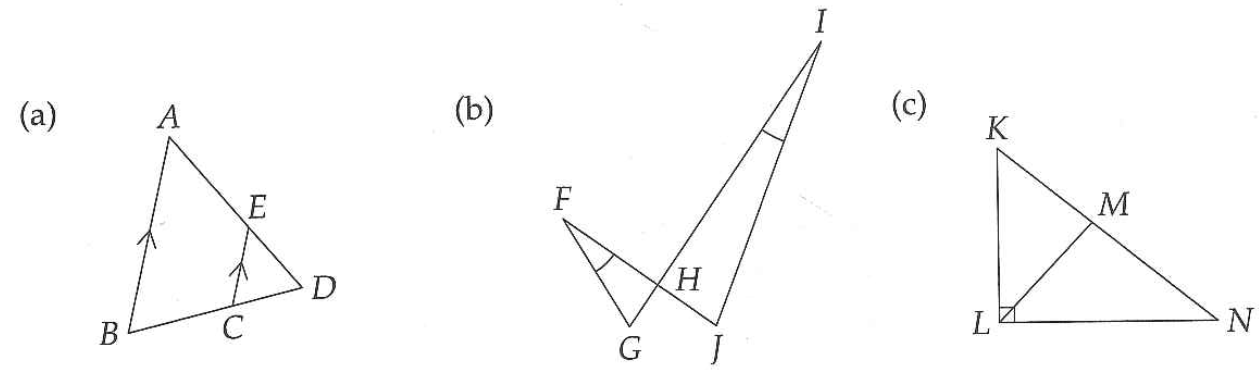
\includegraphics[width=0.9\linewidth]{Geometria/imgs/review_522_1_aopgeo_ejer}
			\label{review_522_1_aopgeo_ejer}
		\end{figure}
		\begin{figure}[H]
			\centering
			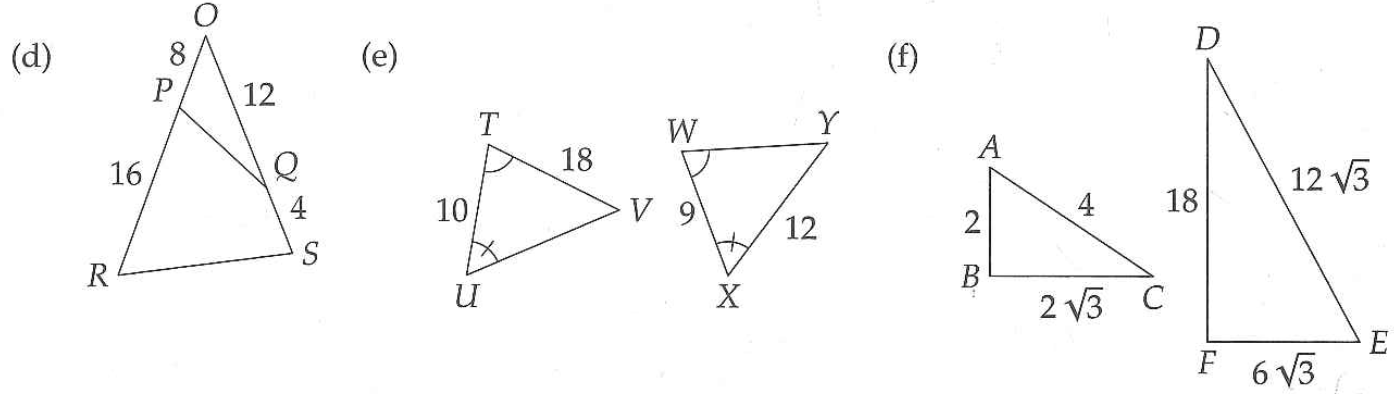
\includegraphics[width=0.9\linewidth]{Geometria/imgs/review_522_2_aopgeo_ejer}
			\label{review_522_2_aopgeo_ejer}
		\end{figure}
		
		\item \label{review_P523_aopgeo_ejercicio} (5.23 de \cite{Aops_Geometria}). En la figura \ref{review_523_aopgeo_ejer}, hallar $x$ e $y$.
			\begin{figure}[H]
				\centering
				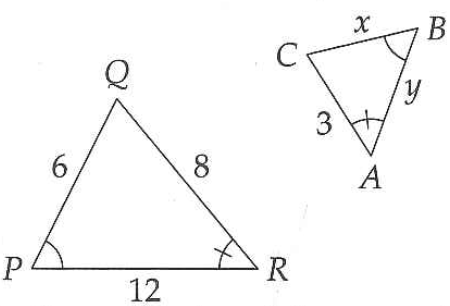
\includegraphics[width=0.4\linewidth]{Geometria/imgs/review_523_aopgeo_ejer}
				\caption{Ejercicio \ref{review_P523_aopgeo_ejercicio}.}
				\label{review_523_aopgeo_ejer}
			\end{figure}
		
		\item \label{review_P524_aopgeo_ejercicio} (5.24 de \cite{Aops_Geometria}). En un $\triangle ABC$, los puntos $P$ y $Q$ están sobre $\overline{AB}$ y $\overline{AC}$ tal que $PQ\parallel BC$. Si $AB=12,PB=9$ y $AC=18$, encontrar $QA$ .
		
		\item \label{review_P525_aopgeo_ejercicio} (5.25 de \cite{Aops_Geometria}). Los lados de un triángulo son 4,6 y 9 centímetros. Uno de los lados de un triángulo similar mide $36cm$. Cuánto es el máximo perimetro que puede tener este otro triángulo?
		
		\item \label{review_P526_aopgeo_ejercicio} (5.26 de \cite{Aops_Geometria}). En la figura \ref{review_523_aopgeo_ejer}, que está mal?
		\begin{figure}[H]
			\centering
			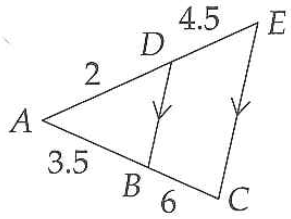
\includegraphics[width=0.35\linewidth]{Geometria/imgs/review_526_aopgeo_ejer}
			\caption{Ejercicio \ref{review_P526_aopgeo_ejercicio}.}
			\label{review_526_aopgeo_ejer}
		\end{figure}
		
		\item \label{review_P527_aopgeo_ejercicio} (5.27 de \cite{Aops_Geometria}). En la figura \ref{review_527_aopgeo_ejer}, hallar $DE$.
		\begin{figure}[H]
			\centering
			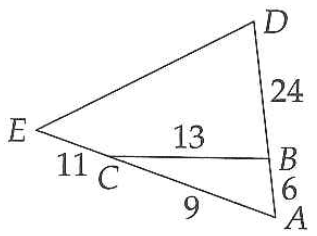
\includegraphics[width=0.3\linewidth]{Geometria/imgs/review_527_aopgeo_ejer}
			\caption{Ejercicio \ref{review_P527_aopgeo_ejercicio}.}
			\label{review_527_aopgeo_ejer}
		\end{figure}
		
		\item \label{review_P528_aopgeo_ejercicio} (5.28 de \cite{Aops_Geometria}). Por qué el diagrama de la figura \ref{review_528_aopgeo_ejer} es imposible?
		\begin{figure}[H]
			\centering
			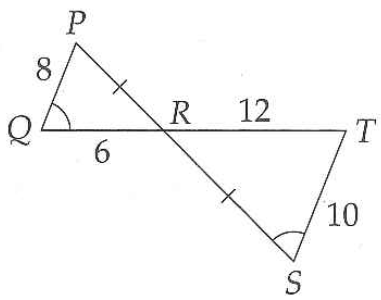
\includegraphics[width=0.4\linewidth]{Geometria/imgs/review_528_aopgeo_ejer}
			\caption{Ejercicio \ref{review_P528_aopgeo_ejercicio}.}
			\label{review_528_aopgeo_ejer}
		\end{figure}
		
		\item \label{review_P529_aopgeo_ejercicio} (5.29 de \cite{Aops_Geometria}). En la figura \ref{review_529_aopgeo_ejer}, hallar $WY$ y $YV$.
		\begin{figure}[H]
			\centering
			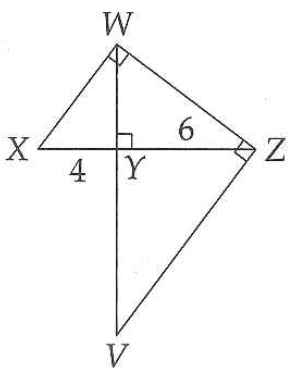
\includegraphics[width=0.3\linewidth]{Geometria/imgs/review_529_aopgeo_ejer}
			\caption{Ejercicio \ref{review_P529_aopgeo_ejercicio}.}
			\label{review_529_aopgeo_ejer}
		\end{figure}
		
		\item \label{review_P530_aopgeo_ejercicio} (5.30 de \cite{Aops_Geometria}). En la figura \ref{review_530_aopgeo_ejer}, $\triangle ABC$ es equilatero.
				\begin{enumerate}[label=\Alph*)]
					\item Probar que $AM=AN$.
					\item Probar que $\triangle AMN$ es equilatero.
				\end{enumerate}
		\begin{figure}[H]
			\centering
			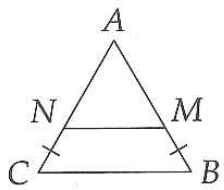
\includegraphics[width=0.28\linewidth]{Geometria/imgs/review_530_aopgeo_ejer}
			\caption{Ejercicio \ref{review_P530_aopgeo_ejercicio}.}
			\label{review_530_aopgeo_ejer}
		\end{figure}
		
		\item \label{review_P531_aopgeo_ejercicio} (5.31 de \cite{Aops_Geometria}). Si $\triangle ABC \sim \triangle YZX$ $[ABC]=40,[YZX]=360,AB=9$ y $BC=12$, hallar:
		\begin{enumerate}[label=\Alph*)]
			\item $YZ$
			\item La longitud de la altura del lado $\overline{XZ}$ del $\triangle YZX$.
		\end{enumerate}
		
		\item \label{review_P532_aopgeo_ejercicio} (5.32 de \cite{Aops_Geometria}). En la figura \ref{review_532_aopgeo_ejer}, $AB=25$ y $BC=12$. Si $AE<BE$ y $\triangle AED \sim \triangle BCE$. Hallar la longitud de $AE$.
		\begin{figure}[H]
			\centering
			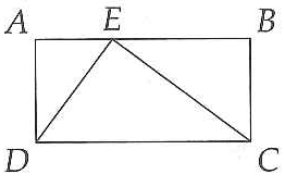
\includegraphics[width=0.35\linewidth]{Geometria/imgs/review_532_aopgeo_ejer}
			\caption{Ejercicio \ref{review_P532_aopgeo_ejercicio}.}
			\label{review_532_aopgeo_ejer}
		\end{figure}
		
		\item \label{review_P533_aopgeo_ejercicio} (5.33 de \cite{Aops_Geometria}). En la figura \ref{review_533_aopgeo_ejer}, $PW=6$ y $WX=4$. Hallar la longitud de $QX$.
		\begin{figure}[H]
			\centering
			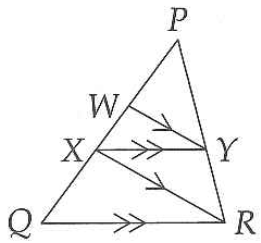
\includegraphics[width=0.35\linewidth]{Geometria/imgs/review_533_aopgeo_ejer}
			\caption{Ejercicio \ref{review_P533_aopgeo_ejercicio}.}
			\label{review_533_aopgeo_ejer}
		\end{figure}
		
		\item \label{review_P534_aopgeo_ejercicio} (5.34 de \cite{Aops_Geometria}). En la figura \ref{review_534_aopgeo_ejer}, $\overline{AP} \parallel \overline{BQ} \parallel \overline{CR}$. Probar que
		\[
				\frac{1}{CR} = \frac{1}{AP} + \frac{1}{BQ}
		\]
		\begin{figure}[H]
			\centering
			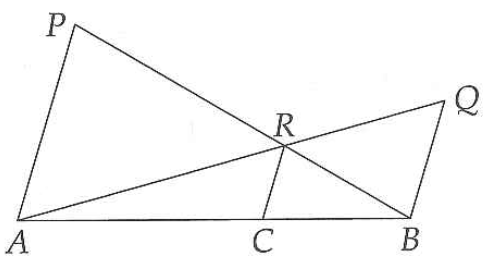
\includegraphics[width=0.45\linewidth]{Geometria/imgs/review_534_aopgeo_ejer}
			\caption{Ejercicio \ref{review_P534_aopgeo_ejercicio}.}
			\label{review_534_aopgeo_ejer}
		\end{figure}
		
		\item \label{review_P535_aopgeo_ejercicio} (5.35 de \cite{Aops_Geometria}). En la figura \ref{review_535_aopgeo_ejer}, dos de los lados del triángulo rectángulo grande miden 20 y12 centímetros. Cuánto mide la altura $h$?
		\begin{figure}[H]
			\centering
			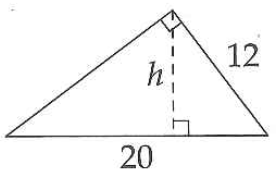
\includegraphics[width=0.4\linewidth]{Geometria/imgs/review_535_aopgeo_ejer}
			\caption{Ejercicio \ref{review_P535_aopgeo_ejercicio}.}
			\label{review_535_aopgeo_ejer}
		\end{figure}
		
		\item \label{review_P536_aopgeo_ejercicio} (5.36 de \cite{Aops_Geometria}). Sea $\triangle ABC$ y sean $D$ y $E$ puntos sobre $\overline{AB}$ y $\overline{AC}$ respectivamente tal que $\overline{DE} \parallel \overline{BC}$. Probar que 
		\[
				\frac{ AD}{AE} = \frac{DB}{CE}
		\]
		
		\item (Tomado de OPM 2017-2018 $2\degree$ eliminatoria, Categoria B problema 2). Sea $\triangle ABC$ de área 9 y $D,E$ y $F$ puntos en los lados $AB, BC$ y $AC$ respectivamente tales que $DE\parallel AC$ y $DF\parallel BC$. Sabiendo que el área de $\triangle DEB$ es cuatro veces el área de $\triangle AFD$, cuál es el área de $\triangle CFE$?	
			\begin{figure}[H]
				\centering
				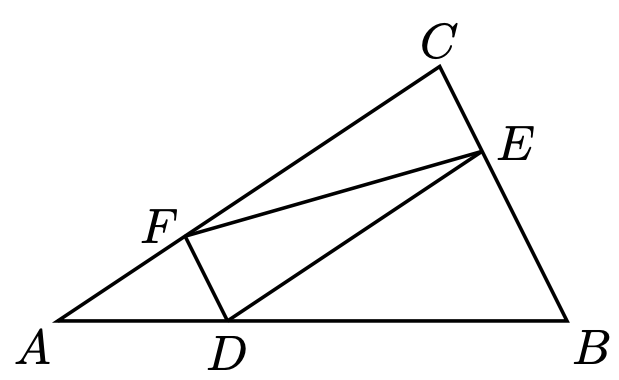
\includegraphics[width=0.45\linewidth]{Geometria/imgs/AV_P4}
				%\caption{}
				\label{avp4}
			\end{figure}
	\end{enumerate}
\newpage

\begin{center}
	\vspace{-1cm}
	\section{ Ejercicios revisión avanzados: Semejanza de triángulos}
\end{center}
\begin{enumerate}
	\item \label{challege_537_aopgeo_ejercicio} (5.37 de \cite{Aops_Geometria}). Sea $ABC$ un triángulo, y sean los puntos $D$ y $E$ sobre $\overline{AB}$ y $\overline{AC}$ respectivamente tales que $\frac{AD}{AE}=\frac{BD}{CE}$. Probar que $\overline{DE} \parallel \overline{BC}$.
	
	\item \label{challege_539_aopgeo_ejercicio}(5.39 de \cite{Aops_Geometria}). En la figura \ref{challege_539_aopgeo_ejer}, $\triangle ABC$ es isosceles, $CH=24cm$, $DE=GF,HF=12cm$ y $FB=6cm$. Encontrar el área de $CDEFG$.
	\begin{figure}[H]
		\centering
		\includegraphics[width=0.4\linewidth]{Geometria/imgs/challege_539_aopgeo_ejer}
		\caption{Ejercicio \ref{challege_539_aopgeo_ejercicio}.}
		\label{challege_539_aopgeo_ejer}
	\end{figure}

	\item \label{challege_540_aopgeo_ejercicio}(5.40 de \cite{Aops_Geometria}). En la figura \ref{challege_540_aopgeo_ejer}, $AD\cdot AC =AE\cdot AB$. Probar que $\angle CDE + \angle CBE = 180\degree$ y $\angle ADB + \angle BEC = 180\degree$.
	\begin{figure}[H]
		\centering
		\includegraphics[width=0.3\linewidth]{Geometria/imgs/challege_540_aopgeo_ejer}
		\caption{Ejercicio \ref{challege_540_aopgeo_ejercicio}.}
		\label{challege_540_aopgeo_ejer}
	\end{figure}
	
	\item \label{challege_541_aopgeo_ejercicio}(5.41 de \cite{Aops_Geometria}). $D,E$ y $F$ están en los lados $\overline{BC}$, $\overline{AC}$ y $\overline{AB}$ recpectivamente del triángulo $ABC$, de forma que $\overline{DE} \parallel \overline{AB}$, $\overline{DF} \parallel \overline{AC}$ y $\overline{BC} \parallel \overline{EF}$. Probar que $D,E$ y $F$ son puntos medios de los lados de $\triangle ABC$.
	
	\item \label{challege_542_aopgeo_ejercicio}(5.42 de \cite{Aops_Geometria}). En la figura \ref{challege_542_aopgeo_ejer}, $\overline{PS} \parallel \overline{QT}$ y $\overline{PQ} \parallel \overline{ST}$. Probar que $\frac{SU}{SP}=\frac{QP}{QR}$.
	\begin{figure}[H]
		\centering
		\includegraphics[width=0.3\linewidth]{Geometria/imgs/challege_542_aopgeo_ejer}
		\caption{Ejercicio \ref{challege_542_aopgeo_ejercicio}.}
		\label{challege_542_aopgeo_ejer}
	\end{figure}

	\item \label{challege_543_aopgeo_ejercicio}(5.43 de \cite{Aops_Geometria}). En la figura \ref{challege_543_aopgeo_ejer}, $[XYZ] = 8$. Los puntos $A$ y $B$ son puntos medios de los segmentos congruentes $\overline{XY}$ y $\overline{XZ}$. La altura $\overline{XC}$ biseca a $\overline{YZ}$. Cuál es el área de la región sombreada?
	\begin{figure}[H]
		\centering
		\includegraphics[width=0.4\linewidth]{Geometria/imgs/challege_543_aopgeo_ejer}
		\caption{Ejercicio \ref{challege_543_aopgeo_ejercicio}.}
		\label{challege_543_aopgeo_ejer}
	\end{figure}

	\item \label{challege_544_aopgeo_ejercicio}(5.44 de \cite{Aops_Geometria}). Al unir los puntos medios de los lados de un triangulo equilatero se construye un segundo triángulo. Un tercer triángulo es construido uniendo los puntos medios de los lados del segundo triángulo. Este proceso se repite hasta construir el décimo triángulo. Cuál es la razón entre las área del décimo triángulo y el tercer triángulo?
	
	\item \label{challege_545_aopgeo_ejercicio}(5.45 de \cite{Aops_Geometria}). En la figura \ref{challege_545_aopgeo_ejer}, $ABCD$ es un rectángulo, $AB=5$ y $BC=3$, $FG=1$ y $GC=2$ . Encontrar el área de $\triangle AEB$.
	\begin{figure}[H]
		\centering
		\includegraphics[width=0.3\linewidth]{Geometria/imgs/challege_545_aopgeo_ejer}
		\caption{Ejercicio \ref{challege_545_aopgeo_ejercicio}.}
		\label{challege_545_aopgeo_ejer}
	\end{figure}

	\item \label{challege_546_aopgeo_ejercicio}(5.46 de \cite{Aops_Geometria}). \textbf{Wow}. En la figura \ref{challege_546_aopgeo_ejer}, $AC=4$ y $BC=3$, $AB=5$ y $\angle ACB=90\degree$ . La secuencia infinita de puntos $C_1,C_2,C_3,C_4\dots$ se forma de la siguiente manera: $C_1$ es el pie de la altura de $C$ sobre $AB$, $C_2$ es el pie de la altura de $C_1$ sobre $AC$, $C_3$ es el pie de la altura de $C_2$ sobre $AB$, y así sucesivamente. Calcular la suma
	\[
			\overline{CC_1} + \overline{C_1C_2}+ \overline{C_2C_3} + \dots 
	\]
	\begin{figure}[H]
		\centering
		\includegraphics[width=0.4\linewidth]{Geometria/imgs/challege_546_aopgeo_ejer}
		\caption{Ejercicio \ref{challege_546_aopgeo_ejercicio}.}
		\label{challege_546_aopgeo_ejer}
	\end{figure}

	\item \label{challege_547_aopgeo_ejercicio}(5.47 de \cite{Aops_Geometria}). \textbf{Wow}. En la figura \ref{challege_547_aopgeo_ejer}, el triángulo grande es equilatero y sus lados se dividen en 4 segmentos congruentes para construir los triángulos equilateros pequeños que se encuentran en el interior. Considere ahora que no se divide en 4 sino en $n$ segmentos congruentes para construir triángulos equilateros pequeños en el interior. Use esto para probar que la suma de los primeros $n$ números impares es $n^2$.
	\begin{figure}[H]
		\centering
		\includegraphics[width=0.3\linewidth]{Geometria/imgs/challege_547_aopgeo_ejer}
		\caption{Ejercicio \ref{challege_547_aopgeo_ejercicio}.}
		\label{challege_547_aopgeo_ejer}
	\end{figure}

	\item \label{challege_548_aopgeo_ejercicio}(5.48 de \cite{Aops_Geometria}). \textbf{Wow}. En la figura \ref{challege_548_aopgeo_ejer}, $AB=6,CD=8,BC=DA=2$ y $\overline{AB} \parallel \overline{CD}$. $P$ es punto medio de $\overline{AB}$, $\overline{PR} \parallel \overline{BC}$ y $\overline{PQ} \parallel \overline{AD}$. Calcular $\frac{PX}{YR}$
	\begin{figure}[H]
		\centering
		\includegraphics[width=0.4\linewidth]{Geometria/imgs/challege_548_aopgeo_ejer}
		\caption{Ejercicio \ref{challege_548_aopgeo_ejercicio}.}
		\label{challege_548_aopgeo_ejer}
	\end{figure}

	\item \label{challege_549_aopgeo_ejercicio}(5.49 de \cite{Aops_Geometria}). \textbf{Wow}. En la figura \ref{challege_549_aopgeo_ejer}, $AF=FG=GB$ y $E$ es punto medio de $\overline{DC}$. $[ABCD]=70$. Hallar el área de $\triangle AHF$.
	\begin{figure}[H]
		\centering
		\includegraphics[width=0.4\linewidth]{Geometria/imgs/challege_549_aopgeo_ejer}
		\caption{Ejercicio \ref{challege_549_aopgeo_ejercicio}.}
		\label{challege_549_aopgeo_ejer}
	\end{figure}

	\item \label{challege_551_aopgeo_ejercicio}(5.51 de \cite{Aops_Geometria}). \textbf{Wow}. En la figura \ref{challege_551_aopgeo_ejer},  $\overline{BC} \parallel \overline{UR}$, $\overline{PS} \parallel \overline{BA}$ y $\overline{TQ} \parallel \overline{AC}$. Probar que
	\[
			\frac{PQ}{BC} + \frac{RS}{CA} + \frac{TU}{AB} = 1
	\]
			\begin{figure}[H]
				\centering
				\includegraphics[width=0.4\linewidth]{Geometria/imgs/challege_551_aopgeo_ejer}
				\caption{Ejercicio \ref{challege_551_aopgeo_ejercicio}.}
				\label{challege_551_aopgeo_ejer}
			\end{figure}
	
	\item (Problema 3 Avanzado OMAPA 2012). 
			\begin{figure}[H]
				\centering
				\includegraphics[width=\linewidth]{Geometria/imgs/OMAPA_AV_2012_P3}
				%\caption{Ejercicio \ref{challege_551_aopgeo_ejercicio}.}
				\label{OMAPA_AV_2012_P3}
			\end{figure}
	
	\item (UK Math Trust Problem of the day 58). En la Figura \ref{UK58} se muestran dos circulos cuyos radios son 3 y 9 unidades, y cuyos centros estan a una distancia de 20 unidades. El segmento $\overline{PQ}$ es tangente a ambos circulos. Cuánto mide $PQ$?
	
			\begin{figure}[H]
				\centering
				\includegraphics[width=0.5\linewidth]{Geometria/imgs/UKMathTrust_PrblemOfTheDay_58}
				%\caption{Ejercicio \ref{challege_551_aopgeo_ejercicio}.}
				\label{UK58}
			\end{figure}
		
	\item (UK Math Trust Problem of the day 66). En la Figura \ref{UK58} calcular el área de toda la figura.
	
	\begin{figure}[H]
		\centering
		\includegraphics[width=0.5\linewidth]{Geometria/imgs/UKMathTrust_PrblemOfTheDay_66}
		%\caption{Ejercicio \ref{challege_551_aopgeo_ejercicio}.}
		\label{UK66}
	\end{figure}

\item (Fase clasificatoria Nivel Avanzado UdeA). 
		\begin{figure}[H]
			\centering
			\includegraphics[width=0.95\linewidth]{Geometria/imgs/udeaproblemasemejanza1}
			%\caption{Ejercicio \ref{challege_551_aopgeo_ejercicio}.}
			%\label{udea1}
		\end{figure}
\end{enumerate}
\newpage


\chapter{Circulos y angulos}
\newpage


\begin{center}
	\vspace{-1cm}
	\section{ Ejercicios: Circulos y ángulos}
\end{center}

\begin{enumerate}	
	\item (Problema 5  Geometría N.2 A.4 de \cite{POTI}). Considere la cricunferencia que circunscribe al triángulo $ABC$. Sea $AE$ un diámetro de esta circunferencia y $AD$ la altura del triángulo en el vértice $A$. Si $AB=6,AC=10$ y $AE=30$. Hallar cuánto mide $AD$.
\end{enumerate}

\newpage
	
	%\input{Geometria/semejanza/semejanza_AV.tex}
	%\input{Geometria/Angulos_en_circulos/circulos_y_angulos.tex}
	

\part{Teoría de Números}
	\chapter{Factorización prima}\label{chapter:factorizacionPrima}

\section{Teorema Fundamental de la Aritmética}\label{section_TFA}
\rule{\textwidth}{0.1mm}
\begin{act}
	Mediante un programa decir si un número es primo o no, luego encontrar los números primos menores que 100 o entre un rango dado.
\end{act}
\rule{\textwidth}{0.1mm}

\textbf{Cuántos números primos existen?}\\


Todo número puede ser factorizado en factores primos, por ejemplo $30=2\cdot3\cdot5$. Cuando aparece más veces un factor primo usamos las potencias, por ejemplo $375=3^1\cdot5^3$.\\

\textbf{Hay algún número que no se pueda descomponer en factores primos?}\\
\textbf{Hay dos números que tengan la misma descomposición en factores primos?}\\

\begin{theorem} \textbf{(Teorema Fundamental de la Aritmética)}\\
	Todo número entero positivo tiene exactamente una única factorización prima. Es decir, dado $a\in {\mathbb{Z}}^{+}$, se tiene que existe una única factorización prima:
	\[a={p_1}^{\alpha_1} \cdot {p_2}^{\alpha_2} \cdot {p_3}^{\alpha_3} \cdots {p_n}^{\alpha_n} \]
\end{theorem}

\textbf{OJO. } Todo número en su descomposición contiene a todos los números primos. Por ejemplo
\[
		375=2^{\color{red}0}\color{black}\cdot 3^1\cdot5^3\cdot 7^{\color{red}0}\color{black}\cdot 11^{\color{red}0}\color{black}\cdot 13^{\color{red}0}\color{black}\cdot 17^{\color{red}0}\color{black}\cdots
\]
\rule{\textwidth}{0.1mm}
\begin{act}
	Mediante un programa hacer la descomposición prima de un número.
\end{act}
\rule{\textwidth}{0.1mm}


\section{Multiplos y MCM}\label{section_multiplos_MCM}
Analicemos los múltiplos en una descomposición prima. 
\begin{center}
\begin{itemize}
	\item $45=\color{red} 3^2\cdot 5^1$
	\item $90=2^1\cdot \color{red} 3^2\cdot 5^1$
	\item $135=3\cdot \color{red} 3^2\cdot 5^1 \color{black}= \color{red} 3^{\color{black}3 }\cdot\color{red} 5^1$
	\item $180=2^2\cdot \color{red} 3^2\cdot 5^1$
\end{itemize}
\end{center}

\textbf{OJO. }La factorización de $mn$, contiene la factorización de $n$ y $m$\\
\textbf{Denotaremos: }$m.c.m\{a,b\}=[a,b]$\\

\begin{ejemplo}
	Encontrar el mínimo común múltiplo de 12 y 45. \\
	\textit{\textbf{Rta:} $[12,45]$ va a ser un número que contiene la factorización de 12 y la de 45, pues es múltiplo de ambos y además es el más pequeño posible. Como $12=\color{blue}2^2\cdot 3^1$ y $45=\color{red}3^2\cdot 5^1$ entonces $[12,45]=\color{blue}2^2\cdot\color{red}3^2\cdot 5^1=\color{black}180$}.
	
	Podemos hallar múltiplos de 180 y así ir encontrando todos los múltiplos comunes de 12 y 45.
\end{ejemplo}

\newpage
\begin{exers}{\ \\}
	\begin{center}
		\vspace{-1cm}
		\subsubsection*{ Mínimo común múltiplo }\label{ejercicios_subsubsection_MCM}
	\end{center}

	\begin{enumerate}
	\item (4.3.1 de \cite{Aops_TN}). Usando la factorización prima encontrar:
				\begin{enumerate}[label=\Alph*)]
					\item $[42,72]$
					\item $[10,56]$
					\item $[9,12,16]$		
				\end{enumerate}
	\item (4.3.3 de \cite{Aops_TN}). Encontrar los primeros 6 múltiplos comunes más pequeños entre 14,15 y 16.
	\item (4.3.4 de \cite{Aops_TN}). Encontrar el menor número de 4 dígitos que sea divisible por 2,3,4,5,6 y 7.
	
	
	\end{enumerate}
\end{exers}
\newpage


Es importante saber hacer y usar la factorización prima, pues esta nos permitirá manipular los enteros para resolver algunos problemas de una forma más rápida. 

\begin{prop}\textbf{(Mínimo común múltiplo)}\\
Dados dos números $a={p_1}^{\alpha_1} \cdot {p_2}^{\alpha_2} \cdot {p_3}^{\alpha_3} \cdots {p_n}^{\alpha_n}$ y $b={p_1}^{\beta_1} \cdot {p_2}^{\beta_2} \cdot {p_3}^{\beta_3} \cdots {p_n}^{\beta_n}$
\[
[a,b]= {p_1}^{\max\{\alpha_1,\beta_1\}} \cdot {p_2}^{\max\{\alpha_1,\beta_1\}} \cdot {p_3}^{\max\{\alpha_1,\beta_1\}} \cdots {p_n}^{\max\{\alpha_1,\beta_1\}}
\]
\end{prop}


\section{Divisores y MCD}\label{section_Divisores_y_MCD}

Así como la factorización permite encontrar los múltiplos, también permite encontrar los divisores.

\begin{ejemplo}\label{Ejemplo_aopsTN_4_11}
	(4.11 de \cite{Aops_TN}). Encontrar la factorización prima de 60 y ver cómo los divisores están relacionados con ella. \\
	\textit{\textbf{Rta:} Podemos ver que $60=2^2\cdot3^1\cdot 5^1$. Por ejemplo 12 es divisor pues $12=\color{red}2^2\cdot 3^1\cdot 5^0$ y $60=\color{red}2^2\cdot 3^1\color{black} \cdot 5^1$}. De la misma forma podemos ver que
		\begin{figure}[H]
			\centering
			\includegraphics[width=0.35\linewidth]{TN/imgs/4_11_aops_tn}
			\caption{Ejemplo \ref{Ejemplo_aopsTN_4_11}}
			\label{4_11_aops_tn}
		\end{figure}
\end{ejemplo}

\textbf{OJO. }La factorización de $n$, contiene la factorización de los divisores de $n$\\
\textbf{Denotaremos: }$m.c.d\{a,b\}=(a,b)$\\

\begin{ejemplo}\label{Ejemplo_aopsTN_4_13}
	Encontrar el máximo  común divisor de 36 y 84. \\
	\textit{\textbf{Rta:} $(36,84)$ va a ser un número que está en la factorización de 36 y en la de 84, pues es divisor de ambos y además es el más grande posible. Como $36=\color{blue}2^2\cdot 3^2$ y $84=\color{red}2^2\cdot 3^1\cdot 7^1$ entonces $(36,84)= 2^2\cdot3^1 =12$}.
	
	Podemos hallar los divisores de 12 y así encontrar todos los divisores comunes de 36 y 84:
	\begin{figure}[H]
		\centering
		\includegraphics[width=0.2\linewidth]{TN/imgs/4_13_aops_tn}
		\caption{Ejemplo \ref{Ejemplo_aopsTN_4_13}}
		\label{4_13_aops_tn}
	\end{figure}
\end{ejemplo}

\newpage
\begin{exers}{\ \\}
	\begin{center}
		\vspace{-1cm}
		\subsubsection*{ Máximo común divisor }\label{ejercicios_subsubsection_MCD}
	\end{center}

	\begin{enumerate}
		\item (4.4.1 de \cite{Aops_TN}). Usando la factorización prima encontrar:
		\begin{enumerate}[label=\Alph*)]
			\item $(12,20)$
			\item $(140,320)$
		\end{enumerate}
		\item (4.4.2 de \cite{Aops_TN}). Encontrar los divisores comunes de 108 y 360.
	\end{enumerate}
\end{exers}
\newpage

\begin{prop}\textbf{(Máximo común divisor)}\\
	Dados dos números $a={p_1}^{\alpha_1} \cdot {p_2}^{\alpha_2} \cdot {p_3}^{\alpha_3} \cdots {p_n}^{\alpha_n}$ y $b={p_1}^{\beta_1} \cdot {p_2}^{\beta_2} \cdot {p_3}^{\beta_3} \cdots {p_n}^{\beta_n}$
	\[
	(a,b)= {p_1}^{\min\{\alpha_1,\beta_1\}} \cdot {p_2}^{\min\{\alpha_2,\beta_2\}} \cdot {p_3}^{\min\{\alpha_3,\beta_3\}} \cdots {p_n}^{\min\{\alpha_3,\beta_n\}}
	\]
\end{prop}

\section{Cuadrados y cubos perfectos}\label{section_cuadrados_cubos_perfectos}

\begin{ejemplo}
	Cómo es la factorización prima de un cuadrado perfecto?\\
	\textit{\textbf{Rta:} Ejemplo, la factorización de $12^2={(2^2\cdot 3^1)}^2=2^4\cdot 3^2$}.
		
	Cuáles de las siguientes descomposiciones son de un cuadrado perfecto? Si no lo son, cuál es el cuadrado perfecto mas grande que lo divide?
	\begin{enumerate}[label=\Alph*)]
	\item $2^8$. 
	\item $2\cdot3^2$. 
	\item $2^{10}\cdot3^2\cdot 5^3$.
	\item $2^2\cdot 7^2$.
	\end{enumerate}
\end{ejemplo}

\begin{ejemplo}
	Cómo es la factorización prima de un cubo perfecto?\\
	\textit{\textbf{Rta:} Ejemplo, la factorización de $18^3={(2^1\cdot 3^2)}^3=2^3\cdot 3^6$}.
	
	Cuáles de las siguientes descomposiciones son de un cubo perfecto? Si no lo son, cuál es el cubo perfecto mas grande que lo divide?
	\begin{enumerate}[label=\Alph*)]
		\item $2^8$. 
		\item $2^3\cdot3^1$. 
		\item $2^{9}\cdot3^3\cdot 5^{13}$.
		\item $2^6\cdot 7^9$.
	\end{enumerate}
\end{ejemplo}

\begin{ejemplo}
	Gina escribe los cubos de tres enteros positivos en un papel. Ricardo dice que cada uno es múltiplo de 18. Gina luego dice que el máximo común divisor de los tres cubos es $n$. Encontrar el valor más pequeño que $n$ puede tener.
\end{ejemplo}

\newpage
\begin{exers}{\ \\}
	\begin{center}
		\vspace{-1cm}
		\subsubsection*{ Descomposición de cuadrados y cubos perfectos }\label{ejercicios_subsubsection_cuadrados_y_cubos_perfectos}
	\end{center}

	
	\begin{enumerate}
		\item (4.6.1 de \cite{Aops_TN}). Encontrar los cinco cuadrados perfectos mas pequeños que son múltipos de 6.
		\item (4.6.3 de \cite{Aops_TN}). Encontrar los seis enteros mas pequeños que son cuadrados perfectos y cubos perfectos.	
		\item (4.6.4 de \cite{Aops_TN}). Encontrar los cuatro cubos perfectos mas pequeños que son múltiplos de 30.
		\item (4.6.5 de \cite{Aops_TN}). Carmelita escribe en una lista el cuadrado perfecto más pequeño que es múltiplo de 20,  el cubo perfecto más pequeño que es múltiplo de 20 y todos los múltiplos de 20 que están entre estos números. Cuántos números hay en la lista de Carmelita?
	\end{enumerate}
\end{exers}
\newpage

\section{Propiedades MCM y MCD}\label{section_propiedades_MCM_MCD}

\begin{ejemplo}\label{Ejemplo_aopsTN_4_20}
	Encontrar $(80n,144n)$ y $[80n,144n]$. \\
\textbf{Rta:} Por ejemplo para cuando $\textbf{n=2}$ tenemos que 
	\begin{equation*}
			\begin{split}
					\textbf{2}\cdot \color{blue} 80 \color{black} &= \textbf{2}\cdot\color{blue}(2^4\cdot3^0\cdot 5^1 )\color{black}=2^5\cdot 3^0\cdot 5^1 \\
					\textbf{2}\cdot \color{red} 144 \color{black}& =\textbf{2}\cdot\color{red}(2^4\cdot3^2\cdot 5^0 )\color{black} =2^5\cdot3^2\cdot 5^0,
			\end{split}
	\end{equation*}
entonces 
	\begin{equation*}
			\begin{split}
					(\textbf{2}\cdot \color{blue} 8\color{black},\textbf{2}\cdot \color{red} 144 \color{black})= 2^5\cdot3^0\cdot 5^0=\textbf{2}\cdot(\color{blue} 8\color{black}, \color{red} 144 \color{black}),
			\end{split}
	\end{equation*}
y
	\begin{equation*}
		\begin{split}
		[\textbf{2}\cdot \color{blue} 8\color{black},\textbf{2}\cdot \color{red} 144 \color{black}]= 2^5\cdot3^2\cdot 5^1=\textbf{2}\cdot[\color{blue} 8\color{black}, \color{red} 144 \color{black}].
		\end{split}
	\end{equation*}
Si hacemos lo mismo para $\textbf{n=3}$, podemos ver que 
	\begin{equation*}
	\begin{split}
	\textbf{3}\cdot \color{blue} 80 \color{black} &= \textbf{3}\cdot\color{blue}(2^4\cdot3^0\cdot 5^1 )\color{black}=2^4\cdot 3^1\cdot 5^1 \\
	\textbf{3}\cdot \color{red} 144 \color{black}& =\textbf{3}\cdot\color{red}(2^4\cdot3^2\cdot 5^0 )\color{black} =2^4\cdot3^3\cdot 5^0,
	\end{split}
	\end{equation*}
	entonces 
	\begin{equation*}
	\begin{split}
	(\textbf{3}\cdot \color{blue} 8\color{black},\textbf{3}\cdot \color{red} 144 \color{black})= 2^4\cdot3^1\cdot 5^0=\textbf{3}\cdot(\color{blue} 8\color{black}, \color{red} 144 \color{black}),
	\end{split}
	\end{equation*}
	y
	\begin{equation*}
	\begin{split}
	[\textbf{3}\cdot \color{blue} 8\color{black},\textbf{2}\cdot \color{red} 144 \color{black}]= 2^4\cdot3^3\cdot 5^1=\textbf{3}\cdot[\color{blue} 8\color{black}, \color{red} 144 \color{black}].
	\end{split}
	\end{equation*}
	Podemos hacerlo sucesivamente y ver que en general
		\begin{equation*}
		\begin{split}
		(\textbf{n}\cdot \color{blue} 8\color{black},\textbf{n}\cdot \color{red} 144 \color{black})=\textbf{n}\cdot(\color{blue} 8\color{black}, \color{red} 144 \color{black}),
		\end{split}
		\end{equation*}
		y
		\begin{equation*}
		\begin{split}
				[\textbf{n}\cdot \color{blue} 8\color{black},\textbf{n}\cdot \color{red} 144 \color{black}]=\textbf{n}\cdot[\color{blue} 8\color{black}, \color{red} 144 \color{black}],
		\end{split}
		\end{equation*}
\end{ejemplo}

\begin{exer}{\ \\}
	(4.21 de \cite{Aops_TN}). Encontrar  $(800,1800)$ y $[800,1800]$.
\end{exer}

\begin{prop}
Dados $a,b$ y $n$ enteros positivos se cumple que 
\begin{enumerate}
		\item $(n\cdot a,n\cdot b)= n\cdot (a,b)$
		\item $[n\cdot a,n\cdot b]= n\cdot [a,b]$		
\end{enumerate}
\end{prop}

\begin{prop}
	Dados $a$ y $b$ enteros positivos se cumple que 
	\[a\cdot b= (a,b)[a,b]\]
\end{prop}

\begin{proof}
	Si $a=P_1^{\alpha_1}\cdot P_2^{\alpha_2}\cdots P_n^{\alpha_n} $ y $b=P_1^{\beta_1}\cdot P_2^{\beta_2}\cdots P_n^{\beta_n} $, entonces 
	\begin{align*}
	(a,b)[a,b] 		&= {p_1}^{\min\{\alpha_1,\beta_1\}} \cdot {p_2}^{\min\{\alpha_2,\beta_2\}} \cdots {p_n}^{\min\{\alpha_n,\beta_n\}} \color{red}\cdot \color{black} {p_1}^{\max\{\alpha_1,\beta_1\}} \cdot {p_2}^{\max\{\alpha_2,\beta_2\}} \cdots {p_n}^{\max\{\alpha_n,\beta_n\}} \\
	&= {p_1}^{\min\{\alpha_1,\beta_1\}} \cdot {p_1}^{\max\{\alpha_1,\beta_1\}} \cdot {p_2}^{\min\{\alpha_2,\beta_2\}} {p_2}^{\max\{\alpha_2,\beta_2\}} \cdots {p_n}^{\min\{\alpha_n,\beta_n\}} \cdot {p_n}^{\max\{\alpha_n,\beta_n\}}\\
	&= {p_1}^{\min\{\alpha_1,\beta_1\} +  \max\{\alpha_1,\beta_1\} }\cdot {p_2}^{\min\{\alpha_2,\beta_2\} + \max\{\alpha_2,\beta_2\}}  \cdots {p_n}^{\min\{\alpha_n,\beta_n\} + \max\{\alpha_n,\beta_n\}} \\
	&= {p_1}^{\alpha_1 + \beta_1} \cdot {p_2}^{\alpha_2 + \beta_2} \cdots {p_n}^{\alpha_n+ \beta_n} \\
	&= P_1^{\alpha_1}\cdot P_1^{\beta_1} \cdot P_2^{\alpha_2}\cdot P_2^{\beta_2}\cdots P_n^{\alpha_n} \cdot P_n^{\beta_n}\\
	&= P_1^{\alpha_1}\cdot P_2^{\alpha_2}\cdots P_n^{\alpha_n} \color{red}\cdot \color{black}  P_1^{\beta_1}\cdot P_2^{\beta_2}\cdots P_n^{\beta_n}\\
	&= a\cdot b
	\end{align*}
\end{proof}












\begin{exer}{\ \\}
	(4.23 de \cite{Aops_TN}). Si el máximo común divisor entre 70 y $n$ es 10 y el mínimo común múltiplo es 210. Encontrar $n$.
\end{exer}

\newpage
\begin{exers}{\ \\}
	\begin{center}
		\vspace{-1cm}
		\subsubsection*{ Propiedades del MCM y MCD }\label{ejercicios_subsubsection_propiedades_de_MCM_MCD}
	\end{center}

	\begin{enumerate}
		\item (4.7.1 de \cite{Aops_TN}). De forma sencilla encontrar 
				\begin{enumerate}[label=\Alph*)]
						\item (50,90)
						\item (750,600)
						\item $[60,70]$
						\item $[444,555]$																		
				\end{enumerate}
		\item (4.7.2 de \cite{Aops_TN}). Encontrar el producto del máximo comun divisor y el mínimo común múltiplo de 100 y 120.
		\item (4.7.3 de \cite{Aops_TN}). Encontrar $n$ si $(n,40)=10$ y $[n,40]=240$.
		\item (4.7.4 de \cite{Aops_TN}). El máximo común divisor entre dos números es 6 y  el mínimo común múltiplo es 450. Si uno de los números es 18, cuál es el otro número?
	\end{enumerate}
\end{exers}
\newpage


\begin{exers}{\ \\}
	\begin{center}
		\vspace{-5mm}
		\section*{Ejercicios de revisión}\label{section_ejercicios_factorizacion_prima_MCM_MCD}
	\end{center}
	\begin{enumerate}
		\item (4.36 de \cite{Aops_TN}). Encontrar $(2520,720)$.
		\item (4.38 de \cite{Aops_TN}). El mínimo común múltiplo de 12,15,20 y $k$ es 420. Cuál es el valor mas pequeño posible que puede tener $k$?
		\item (4.39 de \cite{Aops_TN}). \textbf{Wow}. Un grupo de 10 amigos estan discutiendo sobre un número. ``El se puede dividir por 1" dice el primer amigo. ``El se puede dividir por 2" dice el segundo. ``El se puede dividir por 3" dice el tercero. ``El se puede dividir por 4" dice el cuarto. Continúan así hasta que los diez dicen su comentario.  Si exactamente dos amigos estaban equivocados y estos amigos hablaron de forma consecutiva, cuál es el menor número posible sobre el cuál estaban discutiendo?
		\item (4.40 de \cite{Aops_TN}). \textbf{Wow}. Cuál es el entero positivo $N$ más pequeño tal que el valor $7+30N$ no es un número primo?
		\item (4.41 de \cite{Aops_TN}). Encontrar los cinco múltiplos comunes más pequeños de 18 y 30 que sean cuadrados perfectos y cubos perfectos.				
		\item (4.42 de \cite{Aops_TN}). \textbf{Wow}. El producto de un conjunto de números es 140. Cuál es la suma más pequeña posible que estos pueden tener?		
		\item (4.43 de \cite{Aops_TN}). Encontrar el máximo entero positivo tal que sea divisor de cualquier múltiplo común de 14,26 y 66.
		\item (4.44 de \cite{Aops_TN}). Cuál de los siguientes números tiene el divisor propio más grande: 1999, 2000 o 2001? (Nota: los divisores propios de un número son los divisores sin incluir al mismo número)
		\item (4.45 de \cite{Aops_TN}). 	
						\begin{enumerate}[label=\Alph*)]
							\item Calcular $[24,90]$.
							\item Cualquier múltiplo de 24 y 90 es también múltiplo de 36?
							\item Cualquier múltiplo de 24 y 90 es también múltiplo de 2160?																	
						\end{enumerate}
		\item (4.46 de \cite{Aops_TN}). El más grande de dos números es 8 veces el otro. Explique por qué ambos no pueden ser a la vez cuadrados perfectos?
		\item (4.47 de \cite{Aops_TN}). La suma de los recíprocos de tres números consecutivos es $\frac{47}{60}$. Cuál es la suma de estos tres enteros?
		\item (4.49 de \cite{Aops_TN}). Cuál es el divisor primo más grande de la siguiente serie aritmética:\[1+2+3+\cdots +70?\]
		\item (4.50 de \cite{Aops_TN}). \textbf{Wow.} Encontrar el entero positivo más pequeño que deja residuo 1 cuando se divide por $2,3,\dots,8$ y 9. 
		\item (4.51 de \cite{Aops_TN}). Cuál es el entero positivo más pequeño que al ser multiplicado por 200 es un cubo perfecto?
		\item (4.52 de \cite{Aops_TN}). Juliana escribe los enteros desde 1 hasta 2000 en un papel. Ella borra todos los múltiplos de 3, luego los múltiplos de 5, y así sucesivamente, borrando todos los múltiplos de cada primo impar. Cuántos quedan luego de que termina ?
		\item (4.53 de \cite{Aops_TN}).\textbf{Wow. }Cuántos valores posibles tiene la suma $a+b+c$ si $a,b$ y $c$ son enteros positivos y $abc=72$?
		\item (4.54 de \cite{Aops_TN}). Alex cuenta hasta 400 de 6 en 6 y Mateo cuenta hasta 400 de 4 en 4. Cuántos de los números contados por Alex fueron también contados por Mateo?
		\item (4.55 de \cite{Aops_TN}). Cualquier producto entre dos de los números 30,72 y $N$ es divisible por el tercero. Cuál es el valor mas pequeño posibile que puede tener $N$?
		\item Encontrar todas las parejas de enteros positivos $n$ y $m$ tales que $(n,m)=6$ y $[n,m]=600$.
		
		\item (4.57 de \cite{Aops_TN}). \textbf{Wow}. Bruno, Fernando y Valentina están jugando un juego donde cada carta tiene el número $2,3,4,5,6,7$ o 8. Cada uno se pone la carta en su frente de modo que solo los demás la pueden ver. Juan va caminando y observa que los tres números no son todos diferentes y además que su producto es un cuadrado perfecto. Cuántos de los tres jugadores pueden ahora deducir el número en su frente? 
		
		\item (Selectiva UIS Nivel medio 2020). De los divisores de $5^6\times 7^8$ cuántos son cuadrados perfectos?
		
	\end{enumerate}
\end{exers}
\newpage

\chapter{Divisores: contando divisores, producto de divisores.}\label{chapter:contandoDivisores}

\section{Contando divisores }\label{section:contandoDivisores}


\newpage
\begin{exers}{\ \\}
	\begin{center}
		\vspace{-1cm}
		\subsubsection*{ Contando Dividores }\label{ejercicios:contandoDivisores}
	\end{center}
	
	\begin{enumerate}
		\item (Selectiva UIS Nivel Avanzado 2020). El número \textbf{abab} tiene exactamente 14 divisores. Cuál es el valor de $a+2b$?
		
	\end{enumerate}
\end{exers}
\newpage


\section{Producto de divisores }\label{section:productoDeDivisores}
	%\input{TN/Factorizacion_prima_avanzado/factorizacion_prima_avanzado.tex}
	%\input{TN/Divisores/divisores.tex}
	
\part{Álgebra}\label{algebra}
	\chapter{Ecuaciones lineales de una variable}\label{Capitulo_ecuaciones_lineales_de_una_variable}

\section{Revisión}\label{seccion_revision_ecuaciones_lineales}
Se realizará una revisión del capítulo 3 de \cite{Aops_algebra}.

\begin{ejemplo}{\ \\}
\begin{enumerate}
\item $4x=20$\\
		\textbf{Rta: }$\frac{4x}{4}=\frac{20}{4}$	
		
\item $\frac{a}{9}=\frac{2}{3}$\\
		\textbf{Rta: }
		\begin{align*}
			9\left(\frac{a}{9}\right)&=9\left(\frac{2}{3}\right)\\
			\cancel{9}\left(\frac{a}{\cancel{9}}\right)&=6\\
			a&=6
		\end{align*}

\item $-\frac{2r}{5}=12$\\
		\textbf{Rta: } 
		\begin{align*}
		\left(-\frac{5}{2}\right)\left(\-\frac{2r}{5}\right)&=	\left(-\frac{5}{2}\right)\left(12\right)\\
		r&=-30
		\end{align*}		
\end{enumerate}
\end{ejemplo}

%box de OJO, dato importante
\begin{tcolorbox}[colback=red!5!white,colframe=red!75!black]
El juego es siempre tratar dejar a la variable sola. Si ella va acompañada de un producto, por ejemplo,
\[-\frac{2f}{3}\]
debemos buscar un número que al multplicarlo por $-\frac{2}{3}$ me de $1$, y este es $-\frac{3}{2}$ pues
\[ \left(-\frac{3}{2} \right)\left(-\frac{3}{2}\right)=1 \]
\end{tcolorbox}

\begin{exer}{\ \\}
Resolver la siguientes ecuaciones
\begin{multicols}{3}
\begin{enumerate}[label=\Alph*)]
	\item $-\frac{3s}{8}=-6$
	\item $\frac{x-1}{3}=5$
	\item $3(r-5)=24$
\end{enumerate}
\end{multicols}
\end{exer}

\begin{exer}
Encontrar $a$ si $x=3$ es una solución de la ecuación $\frac{x}{a}=7$.
\end{exer}

\begin{tcolorbox}[colback=red!5!white,colframe=red!75!black]
	Otro truco es \textbf{primero simplificar la ecuación} y luego si resolver. Por ejemplo
	\[3t-7-6+2t=4t+2-6t,\]
	se puede simplificar como $5t-13=-2t-2$ y entonces $7t=11$ y así
	\[t=\frac{11}{7}\]
\end{tcolorbox}

\begin{ejemplo}{\ \\}
\begin{enumerate}
\item Encontrar los valores de $z$ que satisfacen $2z+3-4=3z-5-z$.\\
		\textbf{Rta: }Llegamos a que $-1=-5$, o sea la ecuación no es cierta! Si tenemos una igualdad que no es cierta, entonces todas las anteriores no son ciertas. Es decir, no hay solución.
\item Encontrar los valores de $r$ que satisfacen $3r+5+r=7r-2+7-3r$.
		\textbf{Rta: }Llegamos a que $4r+5=4r+5$, es decir es una igualdad que siempre es cierta independientemente de $r$! o sea hay infinitas soluciones.
\end{enumerate}
\end{ejemplo}

% box de OJO
\begin{tcolorbox}[colback=red!5!white,colframe=red!75!black]
	\begin{itemize}
	\item 	Si llegamos a una igualdad que es falsa, entonces la ecuación no tiene solución.
	\item Si llegamos a una igualdad que es siempre verdadera sin importar la variable, entonces hay infinitas soluciones.
	\end{itemize}
\end{tcolorbox}


\begin{ejemplo}
La ecuación $2x+7=3$ y $bx-10=-2$ tienen la misma solución $x$. Cuál es el valor de $b$?
\end{ejemplo}

\begin{exers}{\ \\}
\begin{enumerate}
\item Resolver las siguientes ecuaciones
		\begin{enumerate}[label=\Alph*)]
		\item $4+2,3y=1,7y-20$.
		\item $-2t+\frac{3}{2} = \frac{t}{4}-12$.
		\item $\frac{x-7}{5}=\frac{x-2}{3}$.
		\end{enumerate}
	
\item Se tiene la la ecuación $3y+2a=4y+7-y+3$.
		\begin{enumerate}[label=\Alph*)]
			\item Para qué valor de $a$ la ecuación tiene infinitas soluciones para $y$?
			\item De un valor de $a$ para el cuál la ecuación no tendría solución.
			\item Cuántos valores puede tener $a$ para que la ecuación no tenga solución.60m
		\end{enumerate}

\end{enumerate}
\end{exers}

\section{Problemas en palabras}\label{seccion_problemas_en_palabras}
La mayoría de problemas de álgebra surgen de la cotidianidad.

\begin{ejemplo}
En este momento soy 3 años mas joven que el doble de la edad que tenía hace 6 años. Cuál es mi edad en este momento?\\
\textbf{Rta: } Es simplemete la ecuación $x=2(x-6)-3$,  de donde se tiene que $x=15$.
\end{ejemplo}

\begin{exers}{\ \\}
\begin{enumerate}
\item (3.3.4 p.73 de \cite{Aops_algebra}). La profesora le dice a Carlos que reste 3 a cierto número y luego divida el resultado por 9. Sin embargo el le resta 9 y luego divide el resultado por 3, lo cual le da como resultado 43. Cuál hubiera sido su respuesta si hubiera resuelto el problema correctamente?

\item (3.3.4 p.73 de \cite{Aops_algebra}). Al final del año 1994 Walter tenía la mitad de la edad que su abuela. La suma de los años en que nacieron es 3838. Cuántos años tendrá Walter al final del año 1999?
\end{enumerate}
\end{exers}

\section{Ecuaciones lineales disfrazadas}\label{Section_ecuaciones_lineales_disfrazadas}
Resolveremos algunas ecuaciones que parece complicadas pero con un simple paso realmente son ecuaciones lineales.

\begin{ejemplo}{\ \\}
\item Encontrar todos los valores de $x$ que satisfagan la ecuación $3\sqrt{x} - 2 = 30-\sqrt{x}$.\\
		\begin{itemize}
		\item \textbf{Forma 1:} Usando una \textbf{\textit{substitución}}. Para que nos quede una ecuación lineal podemos tomar $y=\sqrt{x}$, entonces tenemos
		\[3y-2 = 30-y,\]
		de donde tenemos que $y=8$. Entonces como $y=\sqrt{x}$ entoces $8=\sqrt{x}$ y así vemos que $x=64$.
		
		\item \textbf{Forma 2:} Trabajando con $\sqrt{x}$ como una variable normal. Tenemos $4\sqrt{x}=32$ y entonces $\sqrt{x}=8$ y así calculamos que $x=64$.
		\end{itemize} 
\end{ejemplo}


% box de OJO
\begin{tcolorbox}[colback=red!5!white,colframe=red!75!black]
		Una ecuación díficil a simple vista puede ser convertida en una ecuación lineal que sabemos resolver simplemente haciendo una \textbf{sustitución}. Ejemplo, convertir
		\[3\sqrt{x} - 2 = 30-\sqrt{x},\]
		en
		\[3y-2 = 30-y\]
\end{tcolorbox}

\begin{ejemplo} Resolver la ecuación
\[\frac{3}{x} - 2=7+\frac{2}{x}\]
\begin{itemize}
	\item \textbf{Forma 1:} Para volverlo una ecuación lineal debemos deshacernos de esas $x$ en el denominador, entonces multipliquemos por $x$ la ecuación,
	\begin{align*}
		x \left( \frac{3}{x} - 2 \right) =x \left(7+\frac{2}{x}\right)\\
		\cancel{x} \frac{3}{\cancel{x}} - 2x  =7x+\cancel{x}\frac{2}{\cancel{x}}\\
		3-2x=7x+2\\
		1=9x\\
		\frac{1}{9} = x
	\end{align*}
	Es importante \textbf{comprobar }que la respuesta está bien! Hazlo!
	\item \textbf{Forma 2:} Podemos tomar una \textbf{sustitución}, por ejemplo $y=\frac{1}{x}$.
	\item \textbf{Forma 3:} Trabajando de forma normal.
\end{itemize} 
\end{ejemplo}

\begin{exers}{\ \\}
Juguemos Stop, vamos a resolver las siguientes ecuaciones el que tenga solución diferente suma más puntos.
\begin{enumerate}
\item $\sqrt[3]{2z+1} - 5 + 2 \sqrt[3]{2z+1} = -14$.
\item $2\sqrt{x} +13-\sqrt{r} = 9 - \sqrt{r}$.
\item $\frac{x}{x-1} + \frac{2}{3} = \frac{2}{x-1} $.
\end{enumerate}
\end{exers}

\newpage
\begin{exers}{\ \\}
\begin{center}
	\vspace{-5mm}
	\section*{Ejercicios de revisión}\label{section_ejercicios_ecuaciones_lineales_de_una_variable}
\end{center}
Tomado de p.82-83 de \cite{Aops_algebra}
\begin{enumerate}
\item Resolver las siguientes ecuaciones	
		\begin{multicols}{2}
		\begin{enumerate}[label=\Alph*)]
		\item $\frac{t}{3}-7+\frac{2t}{3}=-3-4$.
		\item $x-3.8x+1.1x=-4.2+2.1x+0.4$.
		\end{enumerate}
		\end{multicols}

\item Una bolsa que contiene reloes pesa 81kg. Cuando 2 relojes se quitan, el peso de la bosa baja a 73kg. La bolsa pesa 1kg cuando está vacía. Cuántos relojes quedan en la bolsa?

\item Resolver las siguientes ecuaciones	
		\begin{multicols}{2}
			\begin{enumerate}[label=\Alph*)]
				\item $\frac{2}{z}+5=\frac{5}{z} -4$.
				\item $\frac{1}{x-1} + \frac{2x}{x-1}=5$.
			\end{enumerate}
		\end{multicols}

\item Hace cinco años, mi abuelo era cinco veces mayor que lo que yo era. Dentro de tres años, mi abuelo va a ser tres veces mayor que lo que yo voy a ser. Que edad tengo en este momento?

\item Cinco enteros consecutivos son sumados. El resultado es 6 mas que el mayor de los cinco enteros. Cuál es el más pequeño de los cinco enteros?

\item Para cual valor de $b$, $x=3$ es una solución de la ecuación $bx^2+3x-2b=0$?

\item Resolver las siguientes ecuaciones	
		\begin{multicols}{2}
			\begin{enumerate}[label=\Alph*)]
				\item $\sqrt[4]{y} + \sqrt[4]{16y}-2=4$.
				\item $\frac{3}{2+\sqrt{y}} + \frac{4}{2+\sqrt{y}} = 1$.
			\end{enumerate}
		\end{multicols}
	
\item \hspace{1cm}	
	\begin{enumerate}[label=\Alph*)]
		\item Sea $x$ el número de en medio de tres enteros consecutivos. Cuál es la suma de estos tres enteros en términos de $x$?.
		\item La suma de 23 enteros consecutivos es 2323. Cuál es el mayor de estos enteros?
	\end{enumerate}

\item Resolver las siguientes ecuaciones	
		\begin{multicols}{2}
			\begin{enumerate}[label=\Alph*)]
				\item $\frac{\sqrt{3+\sqrt[3]{t}}}{\sqrt{3-\sqrt[3]{t}}} = 3$.
				\item $\frac{\sqrt{x+1}+\sqrt{x-1}}{\sqrt{x+1}-\sqrt{x-1}} = 3$.
			\end{enumerate}
		\end{multicols}
\end{enumerate}
\end{exers}
\newpage


\chapter{Mas variables}\label{Capitulo_mas_variables}
Basado en el capitulo 4 de \cite{Aops_algebra}. Al plantear expresiones a veces surge la necesidad de utilizar mas variables.

\begin{ejemplo}
	El triple de la suma de mi edad y la tuya es 4 años más que cuatro veces mi edad. Planteemos una ecuación que represente este problema\\
	\[3(x+y)=4+4x\]
	Se podrá resolver esta ecuación? Que se te ocurre hacer? Si por ejemplo al igual que cuando trabajabamos con una variable intentamos despejar $x$ nos queda
	\[3y-4=x\]
	Cúando esto es cierto? Hay solo un par de valores para los cuales es cierto? o no hay?. Si por ejemplo $x=1$, entonces $y=\frac{5}{3}$. Si $x=2$, entonces $y=2$. Hay infinitas.
\end{ejemplo}

Trabajando con varias variables nos podemos encontrar entonces con muchos tipos de expresiones como

\begin{multicols}{3}
	\begin{itemize}
		\item $\sqrt{x^2+y^2}$
		\item $2a^2b + 3b^2c + 6ac^2$
		\item $\frac{r^2+s^2}{2rs}$
	\end{itemize}
\end{multicols}

\begin{ejemplo}
	En especial, note que si tenemos un triángulo rectángulo donde un cateto mide $x$ y el otro mide $y$, entonces la expresión de cuánto mide la hipotenusa es
	\[ \sqrt{x^2+y^2} \]
\end{ejemplo}

\begin{exer}
	Si decimos que $h$ es la hipotenusa, y $c$ es uno de los catetos, cuál sería la expresión que representa la longitud del otro cateto?
\end{exer}

\begin{exer}
	Evaluar las siguientes expresiones si $a=3/2,b=1$ y $c=6$.
	\begin{multicols}{2}
		\begin{enumerate}
			\item $ab^2c$
			\item $ca^b$
			\item $a^{-1}cb$
			\item $bc^a$
		\end{enumerate}
	\end{multicols}
\end{exer}

\section{Aritmética}\label{capitulo_aritmetica_con_varias_variables}
Al igual que simplificamos expresiones de una variable, podemos simplificar expresiones de más variables.

\begin{ejemplo}
	Simplificando 
	\[
	(5x+5y+3z+3y+3x-15z+2x)
	\]
	tenemos que es lo mismo que
	\[
	10x + 8y +18z
	\]
\end{ejemplo}

\begin{ejemplo}
	Simplificando 
	\[
	\left(3ab-4cd+\frac{3}{2}\right) + \left(2cd - \frac{ab}{2} + 3\right) + (2-ab)
	\]
	tenemos que agrupar los terminos iguales $ab$ y $cd$ :
	\begin{align*}
	\left(3ab-4cd+\frac{3}{2}\right) + \left(2cd - \frac{ab}{2} + 3\right) + (2-ab) &= \left(3ab-\frac{ab}{2} -ab \right) + (2cd -4cd  ) +2 +\frac{3}{2}+ 3 && \text{Agrupando}\\
	&= \frac{6ab-ab-2ab}{2} -2cd + \frac{4+3+6}{2} \\
	&= \frac{3ab}{2}-2cd + \frac{13}{2}
	\end{align*}
	Si tuvieramos por ejemplo $cd$ y $c^2d$ no podríamos agruparlos.
\end{ejemplo}

\newpage
\begin{center}
	\vspace{-5mm}
	\addcontentsline{toc}{subsection}{Ejercicios, Mas variables: Aritmética}
	\subsection*{Ejercicios, Mas variables: Aritmética}\label{section_ejercicios_mas_variables}
\end{center}

\begin{enumerate}
	\item Cuál de las sigueintes opciones es igual a ${(2xy^2)}^5$?
	\begin{multicols}{3}
		\begin{enumerate}[label=\Alph*)]
			\item $2x^5y^{10}$
			\item $64x^6y^7$
			\item $32x^5y^{10}$
		\end{enumerate}
	\end{multicols}
	
	\item Simplificar las siguientes expresiones
	\begin{multicols}{3}
		\begin{enumerate}[label=\Alph*)]
			\item $(3rs^2)\cdot (2rs^3)$.
			\item $\sqrt[3]{27a^6b^3}$.
			\item $\frac{8x^4y^2}{x^3y^3}$.
		\end{enumerate}
	\end{multicols}
	
	\item Simplificar las siguientes expresiones
	\begin{multicols}{3}
		\begin{enumerate}[label=\Alph*)]
			\item $\frac{a}{d} + \frac{3a}{d} + \frac{2}{d} + \frac{2a-2}{d}$.
			\item $(3r^3)(2s^5)(2rs)(4r^2s^3)$.
			\item $\frac{-2x^3y^5z}{-8x^3y^2z^3}$.
		\end{enumerate}
	\end{multicols}
	
	\item Por cuál expresión debo multilicar a $2xt^3$ para obtener $32x^3t^8$?
	
	\item Escriba una expresión para la suma de $k$ enteros positivos comenzando en un entero $n$.
	
\end{enumerate}
\newpage


\section{Distribuir y Factorizar}\label{section_distribuir_y_factorizar}
\begin{tcolorbox}[colback=red!5!white,colframe=red!75!black]
	Recordemos que la \textbf{propiedad distributiva} es
	\[5(t+3s)=5t+15s.\]
	Y lo opuesto es \textbf{factorizar}, es decir 
	\[5t+15s=5(t+3s).\]
\end{tcolorbox}

\begin{ejemplo}{\ \\}
	\begin{enumerate}
		\item Expandir $3xy(x-y)$.
		\item Sacar un factor de $-15ab+35cd$.
		\item Factorizar $7r^2s^2-21rs^3+14rs^4$ 
	\end{enumerate}
\end{ejemplo}

\begin{exer}{\ \\}
	Reducir lo mayor posible la siguente expresión
	\[
	\frac{2x+4y}{8} \cdot \frac{3xy}{x^2+2xy}.
	\]
\end{exer}


Geométricamente podemos ver la factorización de la siguiente forma:
\begin{figure}[h]
	\centering
	\includegraphics[width=0.7\linewidth]{Algebra/imgs/factoratimesMN}
	\caption{Visualización geométrica de la factorización y distribución.}
	\label{fig:factoratimesMN}
\end{figure}



\newpage
\begin{center}
	\vspace{-5mm}
	\addcontentsline{toc}{subsection}{Ejercicios, Mas variables: Distribuyendo y Factorizando}
	\subsection*{Ejercicios, Mas variables: Distribuyendo y Factorizando}\label{ejercicios_section_distribuir_y_factorizar}
\end{center}

\begin{enumerate}
	\item Expandir $(x+y-3z)(2x)$
	
	\item Factorizar las siguientes expresiones
	\begin{multicols}{2}
		\begin{enumerate}[label=\Alph*)]
			\item $3r^3t^2-3r^2t+7r$
			\item $-9a^3c^2+18a^2c^3-3abc$			
		\end{enumerate}
	\end{multicols}
	
	
	\item Reducir lo mayor posible la siguente expresión
	\[
	\frac{2}{3a^2-6b} \cdot \frac{9a^3-18ab}{10a^2}.
	\]
	
	\item Factorizar lo mayor posible la sguente expresión
	\[
	2x(y+1) - 6x^2(y+1)
	\]
	
	\item Expandir $(x+7)(y-4)$
	
\end{enumerate}
\newpage

\section{Fracciones}\label{section_fracciones}
\begin{ejemplo}{\ \\}
	\begin{enumerate}
		\item Simplificar como una fracción fracción
		\[
		\frac{5y}{6x^2} - \frac{4}{3xy}
		\]
		
		\item Simplificar como una fracción fracción
		\[
		\frac{2a^3}{a^3b} + \frac{3b}{a-1} - \frac{3b-3}{6ab-6a}
		\]
		\textbf{Rta: }Antes de podernos a sumar es meojor simplificar antes de buscar una fracción común.
	\end{enumerate}
\end{ejemplo}

\newpage
\begin{center}
	\vspace{-5mm}
	\addcontentsline{toc}{subsection}{Ejercicios, Mas variables: Fracciones}
	\subsection*{Ejercicios, Mas variables: Fracciones}\label{ejercicios_section_fracciones}
\end{center}

\begin{enumerate}
	\item Escribir $\frac{2}{r} + \frac{3}{s}$ como una sola fracción.
	\item Escribir $\frac{2+a}{6ab^2} + \frac{9-b}{9a^2b}$ como una sola fracción.
	\item Escribir $\frac{8r-8s}{2r^2-2rs} + \frac{3r^2}{rs-r}$ como una sola fracción.		
	
\end{enumerate}
\newpage


\section{Ecuaciones}\label{section_ecuaciones}
\begin{ejemplo}{\ \\}
	\begin{enumerate}
		\item Solucionar $x$ en la ecuación $ax=c$ en terminos de $a$ y $c$.
		
		\item Solucionar $x$ en la ecuación $ax+bc=3c-2d^2x$ en terminos de $a,b,c$ y $d$.
	\end{enumerate}
\end{ejemplo}

\newpage
\begin{center}
	\vspace{-5mm}
	\addcontentsline{toc}{subsection}{Ejercicios, Mas variables: Ecuaciones}
	\subsection*{Ejercicios, Mas variables: Ecuaciones}\label{ejercicios_section_ecuaciones}
\end{center}

\begin{enumerate}
	\item Considere la ecuación $\frac{x}{a}+b=c$.
	\begin{enumerate}[label=\Alph*)]
		\item Solucionar la ecuación para $x$ en terminos de $a,b$ y $c$.
		\item Solucionar la ecuación para $b$ en terminos de $a,c$ y $x$.
		\item Solucionar la ecuación para $a$ en terminos de $b,c$ y $x$.										
	\end{enumerate}
	
	\item Solucionar la ecuación $3xy+4=8y-2x$ para $x$ en terminos de $y$.	
	
\end{enumerate}
\newpage


\newpage
\begin{center}
	\vspace{-5mm}
	\addcontentsline{toc}{section}{Ejercicios de Revisión: Varias variables}
	\section*{Ejercicios de Revisión: Varias variables}\label{ejercicios_chapter_varias_variables}
\end{center}

\begin{enumerate}
	\item Simplificar la expresión $2a+3b+7-a+2b+5$ cuando $a=-5b$.
	
	\item Simplifique cada uno de los siuientes:
	\begin{multicols}{2}
		\begin{enumerate}[label=(\Alph*)]
			\item ${(2a^3)}^3 {(3ab^2)}^2$
			\item ${(-2c^3d)}^2 + (4cd^2)(-3c^5)$
			\item $a^3b^3 \sqrt{4a^4b^8}$
			\item $\sqrt[4]{16x^8y^4z^{16}}$
		\end{enumerate}
	\end{multicols}
	
	\item Que expresión se le debe restar a $2x-3y$ para obtener $3x+2y$?
	
	\item Exprese cada uno de los siguientes como una sola fracción:
	\begin{multicols}{2}
		\begin{enumerate}[label=(\Alph*)]
			\item $\frac{1}{a} + \frac{1}{b} + \frac{1}{c}$.
			\item $\frac{3x}{14y^2z^4} + \frac{5y}{18x^3z^2}$.
			\item $\frac{2a^2 - 4a}{3a-6} + \frac{2b^2 - 4b}{8b - 16}$.
			\item $\frac{\frac{3r^2t-6rt^2}{6r^2t^3}}{\frac{8t^3r-4t^2r^2}{6r^3t^4}}$.
		\end{enumerate}
	\end{multicols}
	
	\item Simplificar la expresión $4(x^2 -2y +7) -2(2y^2+4x+2)$ cuando $x=-y$..
	
	\item Por que fracción podemos multiplicar a $\frac{3x^3}{2y^5}$ para obtener $\frac{6y^2}{5x^2}$?
	
	\item
	\begin{enumerate}[label=(\Alph*)]
		\item Expanda el producto $(x-2)(x+2)$.
		\item Factorice la expresión $x^2-y^2$ como producto de dos expresiones tales que ninguna de estas dos es constante.
		
		\item Si $x=\frac{a}{b}$ entonces exprese $\frac{a+b}{a-b}$ en terminos de $x$.
		
		\item \textbf{Wow}. Para que valores de $a$ la ecuación $\frac{6x-a}{x-3} = 3$ no tiene solución para $x$?
		
		\item \textbf{Wow}. Para que valores de $a$ la ecuación $\frac{1}{1+\frac{1}{x}} = a$ no tiene solución para $x$?
		
	\end{enumerate}
\end{enumerate}
\newpage

\chapter{Ecuaciones lineales multivariables}\label{chapter:ecuacionesLinealesMultivaribles}

\begin{ejemplo}
	Consideremos la ecuación 
	\[
	2x-3y = 7
	\]
	Podemos intentar buscar por ensayo y error valores que funcionen. También si tenemos un valor, podemos conocer el otro (ver Tabla \ref{fig:tablaxey}).
	\begin{figure}[h]
		\centering
		\includegraphics[width=0.2\linewidth]{Algebra/imgs/TablaProblemap105}
		\caption{Diferentes valores de $x$ e $y$.}
		\label{fig:tablaxey}
	\end{figure}
	Vemos entonces que $(5,1)$ es una solución a la ecuación. \textbf{Analizando la ecuación:} Notemos que hay un patrón lineal en la forma en que aumentan $x$ e $y$, por que?
	
	\textbf{Rta:} Si aumentamos $x$ en 3, nuestra expresión
	\[
	2x-3y
	\]
	va a aumentar 6, para compensar esto y que nos siga dando 7, tenemos que aumentar $y$ en 2, para que con el $(-3)$ me compense.
	
	Podemos tambien despejar $x$ o $y$ y reemplazar para obtener infinitas soluciones.
\end{ejemplo}

\begin{exer}
	Una solución para la ecuación $3x-5y=-1.9$ es $(x,y) = (1.2,1.1)$. Como podemos hallar otras tres soluciones de forma rápida?
\end{exer}

\section{Sustitución}\label{section:sustitucion}

\begin{ejemplo}
	Solucionar el siguiente sistema de ecuaciones
	\begin{align*}
	x+3y &= 4, \\
	-2x+5y &= -30
	\end{align*}
	Para este tipo de ecuciones podemos aplicar la \textbf{sustitución}, esto es: despejar una variable en una ecuación y reemplazarla en la otra.
\end{ejemplo}


\newpage
\begin{center}
	\vspace{-1cm}
	\addcontentsline{toc}{subsection}{Ejercicios, Ecuaciones lineales multivariables: Sustitución}
	\subsection*{ Ejercicios, Ecuaciones lineales multivariables: Sustitución}\label{ejercicios:sustitucion}
\end{center}

\begin{enumerate}
	\item Solucionar los siguientes sistemas de ecuaciones:
	\begin{multicols}{2}
		\begin{enumerate}[label=\Alph*)]
			\item \begin{align*} 2x+y&=10, \\ 3x-4y &= 37\end{align*}
			\item \begin{align*} \frac{2r}{3}+\frac{5s}{6}&=\frac{11}{2}, \\ \frac{2s}{3}&= \frac{7}{3} + \frac{r}{2}\end{align*}
		\end{enumerate}
	\end{multicols}
	\item Suponga que $x=2-t$ y que $y = 4t+7$.
	\begin{enumerate}[label=\Alph*)]
		\item Si $x=7$, a que es igual $y$?
		\item Si $x=-3$, a que es igual $y$?
		\item Encontrar $y$ en términos de $x$.
	\end{enumerate}
	
	\item En la ecuación
	\begin{align*}
	5x -6y&=1\\
	15x - 18y &= 3
	\end{align*}
	\begin{enumerate}[label=\Alph*)]
		\item Despeje $x$ de le primera ecuación y reemplacelo en la segunda. Al reemplazar, la ecuación es siempre verdadera? Que pares de números cumplen el sistema?
		
		\item Por qué el resultado de la segunda ecuación nos puede indicar que toda pareja que satisface la primera escuación también satisface la segunda?				
	\end{enumerate}
	
	\item Resolver el sistema de ecuaciones 
	\begin{align*}
	13p -92q&=273\\
	12p - 91q &= 273
	\end{align*}
\end{enumerate}
\newpage


%%%%%%%%%%%%%%%%%%%%%%%%%%%%%%%%%%%
%%%%%%%%%%%% ELIMINACIÓN %%%%%%%%%%%%%%%
%%%%%%%%%%%%%%%%%%%%%%%%%%%%%%%%%%%

\section{Eliminación}\label{section:eliminacion}

\begin{ejemplo}
	Solucionar el siguiente sistema de ecuaciones
	\begin{align*}
	2x+3y &= -11, \\
	5x-3y &= 67
	\end{align*}
	Para este tipo de ecuciones podemos aplicar la \textbf{Eliminación}, esto es: sumar las ecuaciones de forma que se eliminen variables.
\end{ejemplo}

\begin{ejemplo}
	Solucionar el siguiente sistema de ecuaciones
	\begin{align*}
	4x-7y &= 13, \\
	2x+3y &= -5
	\end{align*}
	Basta multiplicar la segunda ecuación por $(-2)$. Solución $(x,y) = (2/13, -23/13)$.
\end{ejemplo}

\begin{exer}
	Resolver los siguientes sistemas de ecuaciones
	\begin{multicols}{2}
		\begin{enumerate}[label=\Alph*)]
			\item \begin{align*} 2x+4y&=-9, \\ 2x+6y &= 7\end{align*}
			\item \begin{align*} 5x-2y&=12, \\ x-9y+22 &= -2y\end{align*}
		\end{enumerate}
	\end{multicols}
\end{exer}

\begin{ejemplo}
	Solucionar el siguiente sistema de ecuaciones
	\begin{align*}
	-u+3v &= 8, \\
	10v - 2u &= 16+4v
	\end{align*}
	
	Dividiendo por 2, tenemos entonces que ambas ecuaciones son la misma, entonces cualquier solución de una ecuación también es solucion de la otra. Entonces tenemos infinitas soluciones de $(u,v)$, como las podemos representar?
	\[
	(u,v)=?
	\]
	Entonces podemos darle a $v$ un valor cualquiera, digamos $t$, el cual llamaremos \textbf{parametro}. Entonces tenemos que las \textbf{soluciones paramétricas} son
	\[
	(u,v) = (3t-8,t)
	\]
	así vemos que son infinitas.
\end{ejemplo}

\begin{tcolorbox}[colback=black!5!white,colframe=black]
	\textbf{Aplicando a programación:}
	\begin{itemize}
		\item Para el anterior ejercicio se puede hacer graficando las rectas en geogebra, ver que son la misma.		
	\end{itemize}
\end{tcolorbox}

\begin{tcolorbox}[colback=black!5!white,colframe=black]
	\textbf{Aplicando a programación:} Puedes graficar la solución paramétrica en geogebra, una actividad con esto y mas curvas paramétricas son divertidas para que jueguen parametrizando en geogebra: \textbf{Actividad:} \url{https://www.geogebra.org/m/hhmyprpg} \textbf{Geogebra Class: }\url{https://www.geogebra.org/classroom/uct4pkgw}
\end{tcolorbox}

\begin{ejemplo}
	Solucionar el siguiente sistema de ecuaciones
	\begin{align*}
	-r+2s &= 2, \\
	-2.5r+5s &= 7
	\end{align*}
	Por un lado podemos hacr eliminación y tendríamos una igualdad falsa, entonces no habrían soluciones. Por otro lado podemos ver que ambas ecuaciones son la misma a la izquierda pero en la igualdad no son lo mismo, 
	\begin{align*}
	-5r+10s &= 5, \\
	-5r+10s &= 14
	\end{align*}
	entonces habrá alguna solución de la para este sistema? \textbf{NO!} cualquier solución de una no servirá para la otra. Entonces no hay soución (r,s).
\end{ejemplo}

\begin{exer}{\ \\}
Que valor debe tener $a$ para que hayan infinitas soluciones?
\begin{align*}
-r+2s &= 2, \\
-2.5r+5s &= a
\end{align*}
\end{exer}

\begin{tcolorbox}[colback=red!5!white,colframe=red!75!black]
	Cuando tenemos un sistema de dos ecuaciones hay tres opciones:
	\begin{itemize}
		\item \textbf{No hay solución}. Si llegamos a algo falso, por ejemplo 9=0.
		
		\item \textbf{Una solución}. 
		
		\item \textbf{Infinitas soluciones}. Si llegamos a algo siempre cierto como 0=0, o vemos que ambas ecuaciones son la misma.
	\end{itemize}
\end{tcolorbox}


\newpage
\begin{center}
	\vspace{-1cm}
	\addcontentsline{toc}{subsection}{Ejercicios, Ecuaciones lineales multivariables: Eliminación }
	\subsection*{Ejercicios, Ecuaciones lineales multivariables: Eliminación }\label{ejercicios:eliminacion}
\end{center}

\begin{enumerate}
	\item (p.117 de \cite{Aops_algebra}). Solucionar los siguientes sistemas de ecuaciones:
	\begin{multicols}{2}
		\begin{enumerate}[label=\Alph*)]
			\item \begin{align*} 3x-7y&=14, \\ 2x+7y &= 6\end{align*}
			\item \begin{align*} 5u&=-7-2v, \\ 3u &= 4v-25\end{align*}
			\item \begin{align*} \frac{2x}{13} +2y &= -2(y+1), \\ \frac{-3x}{13}&= -5(6-y)\end{align*}				
			\item \begin{align*} -2.5a +5b &=25, \\ 42+10b &= 15 + 3.75a + 4b\end{align*}				
		\end{enumerate}
	\end{multicols}
	
	\item (p.117 de \cite{Aops_algebra}). Describa todas las soluciones de cada uno de los siguientes sistemas de ecuaciones
	\begin{multicols}{2}
		\begin{enumerate}[label=\Alph*)]
			\item \begin{align*} 2x+3y&=7, \\ 14x &= 49 - 21y\end{align*}
			\item \begin{align*} \frac{3x}{5} - \frac{4y}{5} &= 3, \\ 8y-6x &=5\end{align*}		
		\end{enumerate}
	\end{multicols}
	
	\item Para que valor de de la constante $a$, el siguiente sistema de ecuaciones tiene infinitas soluciones ?
	\begin{align*}
	2x + 5y&= -8\\
	6x &= 16 + a - 15y
	\end{align*}
	
	\item (p.117 de \cite{Aops_algebra}). (\textbf{WOW}). Para que valores de las constantes $a,b,c,d$ y $e$, el siguiente sistema de ecuaciones tiene infinitas soluciones ?
	\begin{align*}
	ax+by&=d\\
	ax+cy&=e
	\end{align*}
\end{enumerate}
\newpage

%%%%%%%%%%%%%%%%%%%%%%%%%%%%%%%%%%%
%%%%%%%% PROBLEMAS DE PALABRAS  %%%%%%%%%%%
%%%%%%%%%%%%%%%%%%%%%%%%%%%%%%%%%%%

\section{Problemas en palabras y mas ecuaciones disfrazadas}\label{section:problemasEnPalabrasyEcuacionesDisfrazadas}

\begin{ejemplo}{\ \\}
	Se jugó un partido de basketball entre dos equipos, Bucaros y Arrieros. Los dos equipos marcaron en total 34 puntos, y los Bucaros ganaron por un margen de 14 puntos. Cuántos puntos marcaron los Arrieros?
	
	\textbf{Solución: }Importante elegir bien el nombre de las variables: ''b`` y ''a`` para el total de puntos maracos por los Bucaros y el total marcado por los Arrieros respectivamente. 
	\begin{align*}
	b + a&= 34\\
	b-b &= 14
	\end{align*}
	Podemos sumar las ecuaciones y resolver facilmente.
\end{ejemplo}

\begin{ejemplo}{\ \\}
	El peso de Juan y dos veces el de Marcos es 361kg y el peso de Marcos y dos veces el de Juan es 362kg. Cuánto pesan Juan y Marcos juntos?
	
	\textbf{Solución: }
	\begin{align*}
	j + 2m&= 361\\
	2j+m &= 362
	\end{align*}
	Sumando, $3j+3m=723$, entonces $j+m=241$.
	\begin{align*}
	b + a&= 34\\
	b-b &= 14
	\end{align*}
	Podemos sumar las ecuaciones y resolver facilmente.
\end{ejemplo}

\begin{ejemplo}{\ \\}
	Hace dos años, Germán tenía nueve veces la edad de Carol. El ahora tiene 7 veces la edad de ella. Cuántos años tienen que pasar desde ahora para que Germán tenga cinco veces la edad de Carol?	
	\textbf{Solución: }
	\begin{align*}
	g&= 7c\\
	g-2 &= 7(c-2)
	\end{align*}
	Sustituyendo $g=7c$, encontramos que $c=8$ y por tanto $g=56$. Para responder la pregunta podemos crear una nueva variable: $t$
	\[56+t = 5(8+t)\]
	de donde tenemos que deben pasar $t=4$ años.
\end{ejemplo}

\begin{exer}{\ \\}
	5 pelotas verdes y dos rojas pesan juntas 10kg, y una pelota verde y 4 rojas pesan juntas 7kg. Si todas las bolas rojas pesan la misma cantidad y todas las verdes pesan lo mismo, cuánto es el peso de 8 pelotas rojas y 8 verdes?
\end{exer}

\begin{exer}{\ \\}
	En cierto momento, Juana nota que su reloj digital marca las dos de la tarde y $a$ minutos. Quince minutos mas tarde el reloj marca las tres y $b$ minutos. Ella se asombra al darse cuenta que $a$ es seis veces mas grande que $b$. Que hora era cuando ella vió el reloj por segunda vez?
\end{exer}

\begin{ejemplo}{\ \\}
	Encontrar todos los posibles valores de $a$ y $b$ tales que la suma de sus raices cuadradas sea 37 y la raiz cuadrada de $a$ sea 10 mas que el doble de la raiz de $b$.
	
	\textbf{Solución: }
	\begin{align*}
	\sqrt{a} + \sqrt{b}&= 37\\
	\sqrt{a}&= 2\sqrt{b}+10
	\end{align*}
	Podemos continuar solucionandolo así. Pero que sería mas sencillo solucionar
	\begin{align*}
	r + s= 37\\
	r &= 2s+10
	\end{align*}
	Teniamos entonces una ecuacion lineal disfrazada. De donde obtenemos $r=28$ y $s=9$, entonces $a=28^2$ y $b=9^2$.
\end{ejemplo}

\begin{ejemplo}{\ \\}
	Encontrar todas las parejas $(x,y)$ que satisfacen la siguiente ecuación
	\begin{align*}
	\frac{3}{x} - \frac{2}{y} &= -\frac{7}{2}\\
	\frac{6}{x} + \frac{4}{y} &= 9
	\end{align*}
	
	\textbf{Solución 1: }
	Para deshacernos de los denominadores,
	\begin{align*}
	2xy \left( \frac{3}{x} - \frac{2}{y} \right) &= 2xy\left( -\frac{7}{2} \right)\\
	xy \left( \frac{6}{x} + \frac{4}{y} \right) &= xy\left( -9 \right)
	\end{align*}
	Entonces tenemos
	\begin{align*}
	-4x+6y&=-7xy \\
	4x+6y&=9xy
	\end{align*}
	sumando tenemos $12y=2xy$, podemos dividir por $y$? Si! pues $y$ no puede ser cero. Entonces $x=6,y=1/2$.
	
	\textbf{Solución 2: }
	Para evitar trabajar con los reciprocos $1/x$ y $1/y$ podemos usar otras variables para ellos, $r$ y $s$ respectivamente, entonces
	\begin{align*}
	3r -2s&=  -\frac{7}{2} \\
	6r + 4s &= -9 
	\end{align*}
	este sistema es mucho mas fácil y podemos encontrar la solución $(r,s)=(1/6,2)$, entonces $(x,y)=(6,1/2)$.
	
	\textbf{Solución 3: }
	Si te detienes un poco a pensar puede ver que multiplicando la primera ecuación por 2 nos deja $-4/y$ en la primera y $4/y$ en la segunda,
	\begin{align*}
	\frac{6}{x} - \frac{4}{y} &= -7\\
	\frac{6}{x} + \frac{4}{y} &= 9
	\end{align*}
	sumando tenemos $12/x = 2$, entonces $x=6$.		
\end{ejemplo}

\newpage
\begin{center}
	\vspace{-1cm}
	\addcontentsline{toc}{subsection}{Ejercicios, Ecuaciones lineales multivariables: Problemas en palabras y mas ecuaciones disfrazadas }
	\subsection*{Ejercicios, Ecuaciones lineales multivariables: Problemas en palabras y mas ecuaciones disfrazadas.}\label{ejercicios:part:algebra:chapter:problemasEnPalabrasyEcuacionesDisfrazadas}
\end{center}	
\begin{enumerate}
	\item (p.125 \cite{Aops_algebra}). Resolver el sistema de ecuaciones para $x$ e $y$.
	\begin{align*}
	\frac{6}{x} + \frac{7}{y} &= 4\\
	\frac{2}{x} -  \frac{5}{y} &= 16
	\end{align*}
	\item (p.126 \cite{Aops_algebra}). La suma de las areas de dos cuadrados es 65, mientras que la diferencia en sus areas es 33. Encontrar la suma de sus perimetros
	
	\item (p.126 \cite{Aops_algebra}). \textbf{Wow}. Encontrar $r$ y $s$ si $\sqrt[3]{r}+ 9\sqrt{s} =21$ y $10 \sqrt[3]{r} - \sqrt{s} =28$
	
\end{enumerate}
\newpage

%%%%%%%%%%%%%%%%%%%%%%%%%%%%%%%%%%%
%%%%%% PROBLEMAS DE MAS VARIABLES  %%%%%%%%%%
%%%%%%%%%%%%%%%%%%%%%%%%%%%%%%%%%%%

\section{Problemas con mas variables }\label{section:problemas_con_mas_variables}

\begin{ejemplo}{\ \\}
	Resolver el sistema de ecuaciones
	\begin{align*}
	x+3y-4z &= 25\\
	-2x+5y+7z &= -66\\
	3x-2y+3z &= 7
	\end{align*}
	\textbf{Solución: }Tratemos de convertirlo en un problema que conozcamos. De la primera ecuación $x=25-3y+4z$ podemos reemplazarla en las otras dos para solucionar y poder calcular $y$ e $z$. De donde podemos calcular $y=-2$, $z=-6$ y con esto podemos calcular $x$, que sería $7$. Entonces la solución es $(x,y,z) = (7,-2,-6)$.
\end{ejemplo}

\begin{tcolorbox}[colback=red!5!white,colframe=red!75!black]
	\textbf{Sustituir} es una herramienta útil para solucionar problemas con muchas variables.
\end{tcolorbox}

\begin{ejemplo}{\ \\}
	Resolver el sistema de ecuaciones
	\begin{align*}
	2x-3y+6z &= -12\\
	5x+2y-8z &= 29\\
	7x+6y+4z &= 49
	\end{align*}
	\textbf{Solución: } Aquí no podemos sustituir sin involucrarnos con fracciones, lo cual es un poco incómodo. Podemos entonces eliminar la variable que queramos,
	\begin{align*}
	4x-6y+12z &= -24 \quad \text{multiplicamos por 2}\\
	15x+6y-24z &= 87 \quad \text{multiplicamos por 3}\\
	7x+6y+4z &= 49
	\end{align*}
	de las primera dos ecuaciones tenemos $19x-12z=63$ y de la primera y tercera $11x +16z=25$. Redujimos entonces el problema a
	\begin{align*}
	19x-12z &= 63\\
	11x +16z &= 25
	\end{align*}
	De acá nuevamente eliminando, podemos encontrar $x=3$ y $z=-1/2$. Entonces la solución es $(x,y,z) = (3,5,-1/2)$.	
\end{ejemplo}

\begin{ejemplo}{\ \\}
	En la tienda de las vocales, cada vocal se vende a diferente precio, pero todas las consonantes son gratis. La palabra ``triangle'' se vende a $\$ 6$, ``square'' a $\$ 9$, ``pentagon'' a $\$ 7$, ``cube'' a $\$ 7$ y ``tetrahedron'' a $\$8$. Cuánto cuesta la palabra ``octahedron''?
	\textbf{Solución: } 
	\begin{align*}
	a+e+i &= 6\\
	a+e+u &= 9\\
	a+e+o &= 7\\
	e+u &= 7 \\
	a+2e+o &= 8
	\end{align*}
	De la segunda y cuarta ecuación tenemos que $a=2$. Entonces ahora tenemos
	\begin{align*}
	e+i &= 4\\
	e+u &= 7\\
	e+o &= 5\\
	2e+o &= 6
	\end{align*}
	Restanto la segunda ecuación de la cuarta, tenemos $e=1$, y con esto ya podemos saber el valor de las otras vocales: $i=3,u=6$ y $o=4$. Entonces la solución de las ecuaciones es $(a,e,i,o,u) = (2,1,3,4,6)$.Y por tanto ``octahedron'' cuesta $\$ 11$.
\end{ejemplo}

\newpage

\begin{center}
	\vspace{-1cm}
	\addcontentsline{toc}{subsection}{Ejercicios, Ecuaciones lineales multivariables:Problemas con mas variables. }
	\subsection*{ Ejercicios, Ecuaciones lineales multivariables:Problemas con mas variables.}
\end{center}	
\begin{enumerate}
	\item (p.130 \cite{Aops_algebra}). Encontrar todas las soluciones del siguiente sistema de ecuaciones 
	\begin{align*}
	x+3y+2z &= 6\\
	-3x+y+5z &= 29\\
	-2x-3y+z &= 14
	\end{align*}
	
	\item (p.131 \cite{Aops_algebra}). Encontrar todas las soluciones del siguiente sistema de ecuaciones 
	\begin{align*}
	2x-5y+3z &= 25\\
	-x-y+4z &= -6\\
	3x + 3y -z &= -4
	\end{align*}
	
	\item (p.131 \cite{Aops_algebra}). En el cuadrado mágico que se muestra en la Figura \ref{fig:cuadrado_magico}, la suma de los números en cada fila, columna y diagonal es la misma. Encontrar el valor de $y+z$
	\begin{figure}[H]
		\centering
		\includegraphics[width=0.25\linewidth]{Algebra/imgs/cuadrado_magico.png}
		%\caption{_caption_}
		\label{fig:cuadrado_magico}
	\end{figure}
	
	\item (p.131 \cite{Aops_algebra}). 	Considere el siguiente sistema de ecuaciones
	\begin{align*}
	2a+3b-4c &= 7\\
	a-b+2c &= -6
	\end{align*}
	\begin{enumerate}[label=(\Alph*)]
		\item Encontrar una solución $(a,b,c)$ que satisfaga ambas ecuaciones.
		\item Puede encontrar usted otra tripleta $(a,b,c)$ que satisfaga ambas ecuaciones?
		\item Solucionar $b$ en términos de $a$ y $c$ en terminos de $a$. Cuántas soluciones tiene este sistema?
	\end{enumerate}
	
\end{enumerate}
\newpage


\newpage
\begin{center}
	\vspace{-5mm}
	\addcontentsline{toc}{section}{Ejercicios derevisión: Ecuaciones lineales multivariables}
	\section*{Ejercicios de revisión: Ecuaciones lineales multivariables }\label{section:label_section}
\end{center}

\begin{enumerate}
	\item (p.133 \cite{Aops_algebra}). Encuentre tres parejas $(a,b)$ que satisfagan la ecuación $3a-5b=9$.
	
	\item (p.133 \cite{Aops_algebra}).Utilice \textbf{sustitución} para resolver el siguiente sistema de ecuaciones
	\begin{align*}
	x+4y &= -5\\
	3x-8y&=45
	\end{align*}
	
	\item (p.133 \cite{Aops_algebra}).Utilice \textbf{sustitución} para resolver el siguiente sistema de ecuaciones
	\begin{align*}
	3a-b&= 11\\
	6a+4b&=1
	\end{align*}
	
	\item (p.133 \cite{Aops_algebra}).Utilice \textbf{eliminación} para resolver el siguiente sistema de ecuaciones
	\begin{align*}
	5x-6y &= -64\\
	7x+3y&= -44
	\end{align*}
	
	\item (p.133 \cite{Aops_algebra}).Utilice \textbf{eliminación} para resolver el siguiente sistema de ecuaciones
	\begin{align*}
	3x-8y &= -7\\
	6x+16y&= 4
	\end{align*}
\end{enumerate}
\newpage
	%\input{Algebra/Ecuaciones_lineales_una_variable/Avanzado_Revision_Ecuaciones_lineales_una_variable.tex}
	
	%\input{Algebra/mas_variables/cam_variables_AV.tex}
	
	%\input{Algebra/EcuacionesLinealesMultivariables/EcuacionesLinealesMultivariables.tex}
%----------------------------------------------------------------------------------------
%----------------------------------------------------------------------------------------
%-----------------                            SOLUCIONES                       ----------------------
%----------------------------------------------------------------------------------------
%----------------------------------------------------------------------------------------
\part{Soluciones}
\chapter{Combinatoria}\label{sol:chapter:combinatoria}


\chapter{Geometr\'ia}\label{sol:chapter:geometria}


\chapter{Teor\'ia de N\'umeros}\label{sol:chapter:teoria_de_numeros}


\chapter{\'Algebra}\label{sol:chapter:algebra}
%\chapter{Algebra}	
%\input{Algebra/Solucion_algebra.tex}

		
\begin{thebibliography}{9}
	\bibitem{ICP_Aops}
	David Patrick. \textit{Introduction to Counting and Probability}. Aops, 2005.
	
	\bibitem{Aops_Geometria}
	\textit{Introduction to Geometry (AOPS)}
	
	\bibitem{Aops_algebra}
	\textit{Introduction to Algebra (AOPS)}
	
	\bibitem{Contagem_e_probabilidade}
	Paulo Cezar Pinto Carvalho. \textit{Métodos de Contagem e Probabilidade}, IMPA, OBMEP.
	
	\bibitem{clemens}
	Standley R. Clemens y Phares G O'Daffer \textit{Geometría}, Addison Wesley Longman
	
	\bibitem{POTI}
	Programa Olímpico de Treinamento
	
	\bibitem{Aops_TN}
	\textit{Introduction to Number Thoery (AOPS)}
	
	\bibitem{Dimensions_Math_7A}
	Dimensions Math 7A \textit{a Singapore Math Program} 
\end{thebibliography}



\end{document}